\chapter{Signal Simulation}\label{ch:signal}

This analysis is searching for large extra-dimensional signals as described by the ADD model. This BSM signal produces a nonresonant excess over the SM diphoton background and is modeled using MC simulation. A large parameter space is considered in the search.

\section{Signal Generation}\label{sec:ADD_gen}

For this search, the final state of ADD signal comes from the excited state of the \KK graviton decaying to two high-mass photons ($\Gkk \to \gamma\gamma$). This final state is initiated through quark annihilation and gluon fusion at the LHC, as depicted in the Feynman diagrams in Fig.~\ref{signal_diagrams}, and is mediated by virtual graviton exchange. Since proton-proton collisions are used at the LHC, the gluon-initiated processes dominate over the quark-initiated ones, due to the larger gluon contribution to the proton PDFs, as previously shown in Fig.~\ref{fig:ct10_pdf}.

Similar to the real background calculation, the ADD signal is calculated with the MC event generator \SHERPA~v.2.1.1 using the CT10 set of PDFs. In order to account for the large interference effects between the ADD signal and SM background, discussed in Chapter~\ref{ch:intro}, the ADD signal MC samples are generated in conjunction with the SM diphoton background processes in the high-\Mgg region considered here. However, it is not computationally feasible to generate the combined signal and background processes together at high orders, so only the LO background processes are considered. Hence, unlike the background calculation, no additional final state jets are added to the Born diagrams for the signal generation. This yields samples containing the combined ADD signal and SM background processes, which we denote ADD\texttt{+}SM. \correction{As explained in Chapter~\ref{ch:background}, the inclusion of the additional jets primarily affects the sampling of the angular phase space.}

 \correction{Even though the additional final state jets are absent in the ADD\texttt{+}SM samples, what is important is extracting the final ADD signal (which includes the interference effects) in an appropriate manner. This is done by generating separate SM-only background samples that are identical to the ADD\texttt{+}SM samples, but exclude the ADD signal contribution.} These SM-only samples allow us to subtract the SM background from the ADD\texttt{+}SM samples yielding the final samples containing only the contributions from the signal and the interference effects, which are needed for the limit setting procedure discussed in Chapter~\ref{ch:results}. \correction{When validating this approach, some samples were able to be produced with the inclusion of one additional jet. The \mgg shapes of the final distributions using one additional jet matched those produced using no additional jets.}

The implementation of the ADD model within \SHERPA~\cite{Gleisberg:2003ue} is parameterized by the string cutoff scale \Ms and the number of extra dimensions \nED. In this implementation, the cutoff scale \Ms is related to the fundamental Planck scale \MD by
\begin{equation}
	\Ms = 2\sqrt{\pi}\left[\Gamma(\nED/2)\right]^{1/(\nED+2)}\MD
\end{equation}
\noindent where $\Gamma$ is the gamma function. Since the cross section is cutoff at \Ms, the \Mgg distribution is truncated at the chosen value of \Ms during signal generation. This conservative estimate sets the cross section to zero above \Mgg. Each of the three cutoff conventions, GRW, HLZ, and Hewett, as discussed in Chapter~\ref{ch:intro}, are separately considered. Note, another common choice for the cutoff scale is the mass scale \LambdaT, which can be related to \Ms. For example, in the GRW convention, $\Ms = \LambdaT$ for virtual graviton exchange processes, while for real graviton emission processes $\Ms = \MD$.

These different conventions are implemented in \SHERPA and can be selected by choosing an appropriate value for the internal parameter \KK. Using $\KK=0$, the constant mass parameter, the contributions from the ADD signal during generation are effectively turned off, leaving just the SM background without any interference. Both $\KK=1$ and $\KK=2$ correspond to the HLZ convention with $\KK=1$ being the ``simplified" sum and $\KK=2$ being the ``exact" sum of the internal \KK propagators. The simplified sum is a LO approximation and is specified in the corresponding term in Eq.~(\ref{eqn:add_f_conventions}). This form is typically quoted in the literature, including previous CMS searches, and is considered in this analysis. The Hewett convention offers both positive ($\mathcal{F} = +\frac{2}{\pi}$) and negative ($\mathcal{F} = -\frac{2}{\pi}$) interference scenarios. The value $\KK=3$ is used to select Hewett with positive interference (Hewett\texttt{+}) and $\KK=4$ is used for Hewett with negative interference (Hewett\texttt{-}). The GRW convention is specified using $\KK=5$. These are summarized as follows:

\begin{itemize}
	\item $\KK=0$ $\rightarrow$ constant mass;
	\item $\KK=1$ $\rightarrow$ HLZ (simplified);
	\item $\KK=2$ $\rightarrow$ HLZ (exact);
	\item $\KK=3$ $\rightarrow$ Hewett\texttt{+};
	\item $\KK=4$ $\rightarrow$ Hewett\texttt{-}; and
	\item $\KK=5$ $\rightarrow$ GRW.
\end{itemize}


\section{The ADD Convention Relations}

As an illustration, the signal was generated for Hewett\texttt{+} using $\Ms = 4000\GeV$ and its diphoton invariant mass \Mgg distribution is shown in Fig.~\ref{fig:ADD_with_SM}. This distribution includes the total combined signal, background, and interference components. Notice \Mgg is cut off at $\Ms = 4000\GeV$. This is compared against the invariant mass from only the SM background (also truncated at $\Mgg = 4000\GeV$ for illustration). Note, to improve statistics, the generation was done in \Mgg bins of 500-1000, 1000-2000, and 2000-4000\GeV, but some statistical fluctuations can still be observed near the bin edges. In this case, the SM background was generated by specifying $\KK=0$. Both distributions are normalized to have cross sections of 1\fbinv. The nonresonant ADD signal enhancement over SM background is evident at high mass.

\begin{figure}[!htbp]
  \centering
  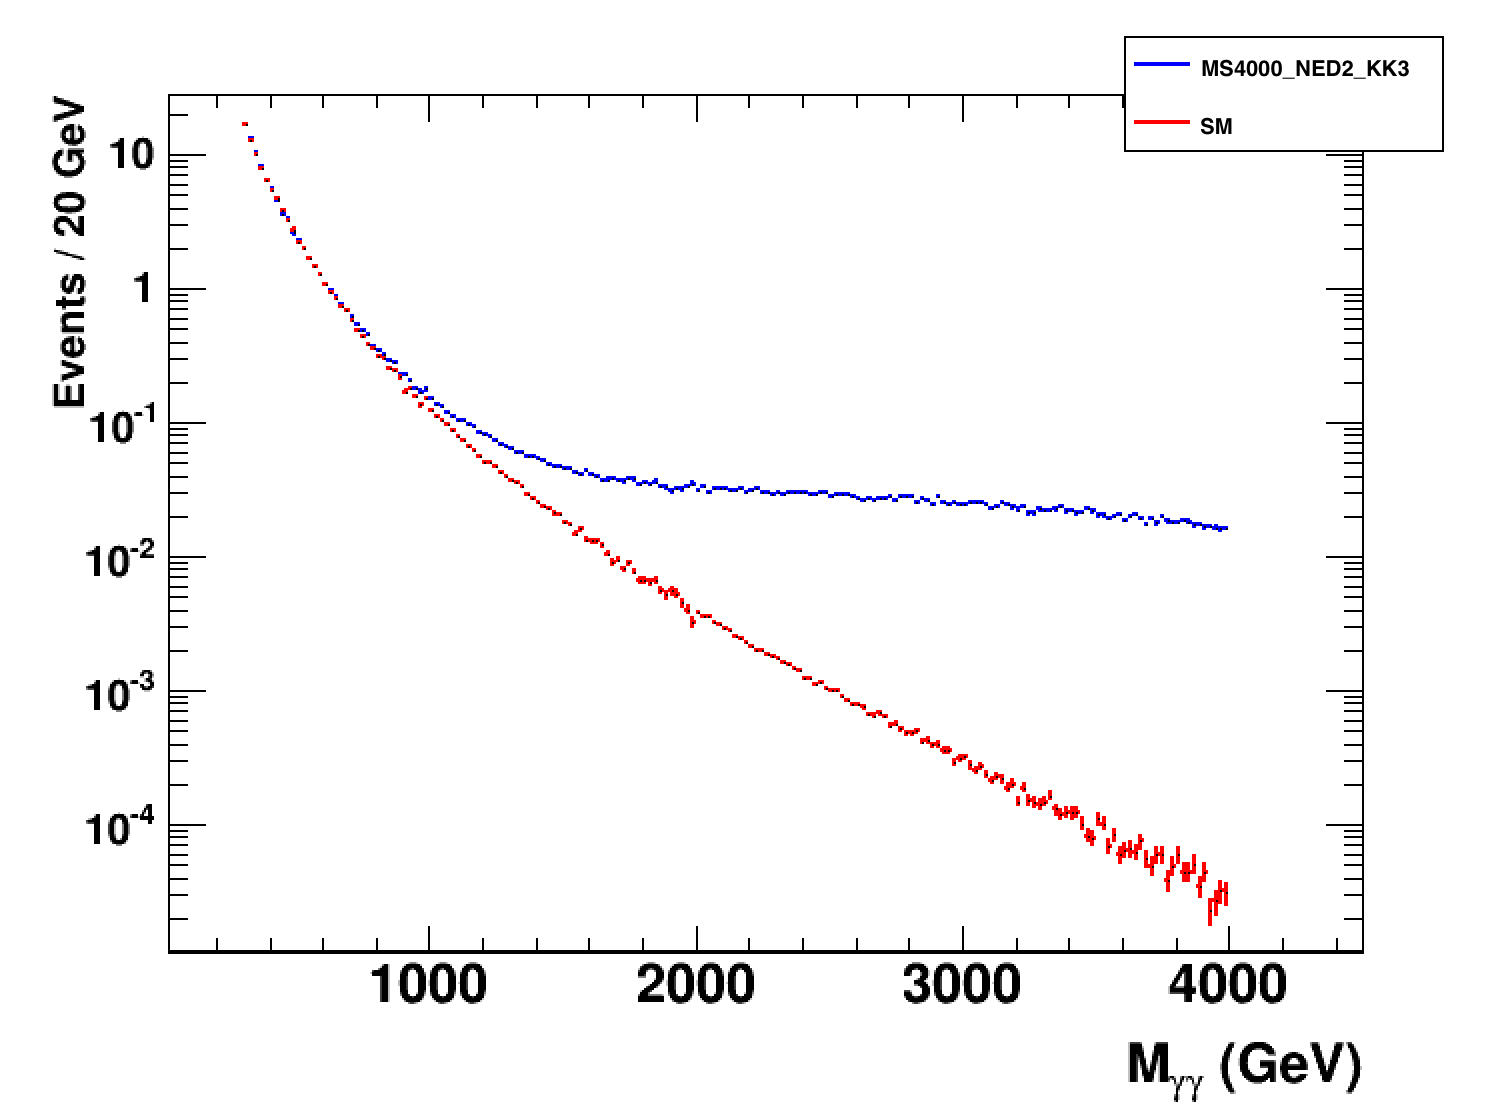
\includegraphics[width=0.75\textwidth]{figures/Hewett_pos_with_SM_Bkg}
  \caption{The \mgg distributions for the ADD signal using the Hewett\texttt{+} convention with $\Ms = 4000\GeV$ (blue) compared to the SM background (red).}
  \label{fig:ADD_with_SM}
\end{figure}

Fig.~\ref{fig:ADD_photon_eta} compares photon $\eta$ of the combined ADD\texttt{+}SM distributions from the GRW convention at values of $\Ms = 2000$, 4000, and 6000\GeV against that of only the SM background. The signal compared to background tends to be peaked in the central region of $\eta$. This allows for more sensitivity in the barrel region of the detector over the endcap, in particular, in the EB. We see for larger values of \Ms, the signal appears more SM like, as expected since the SM background is recovered as $\Ms \to \infty$.

\begin{figure}[!htbp]
  \centering
  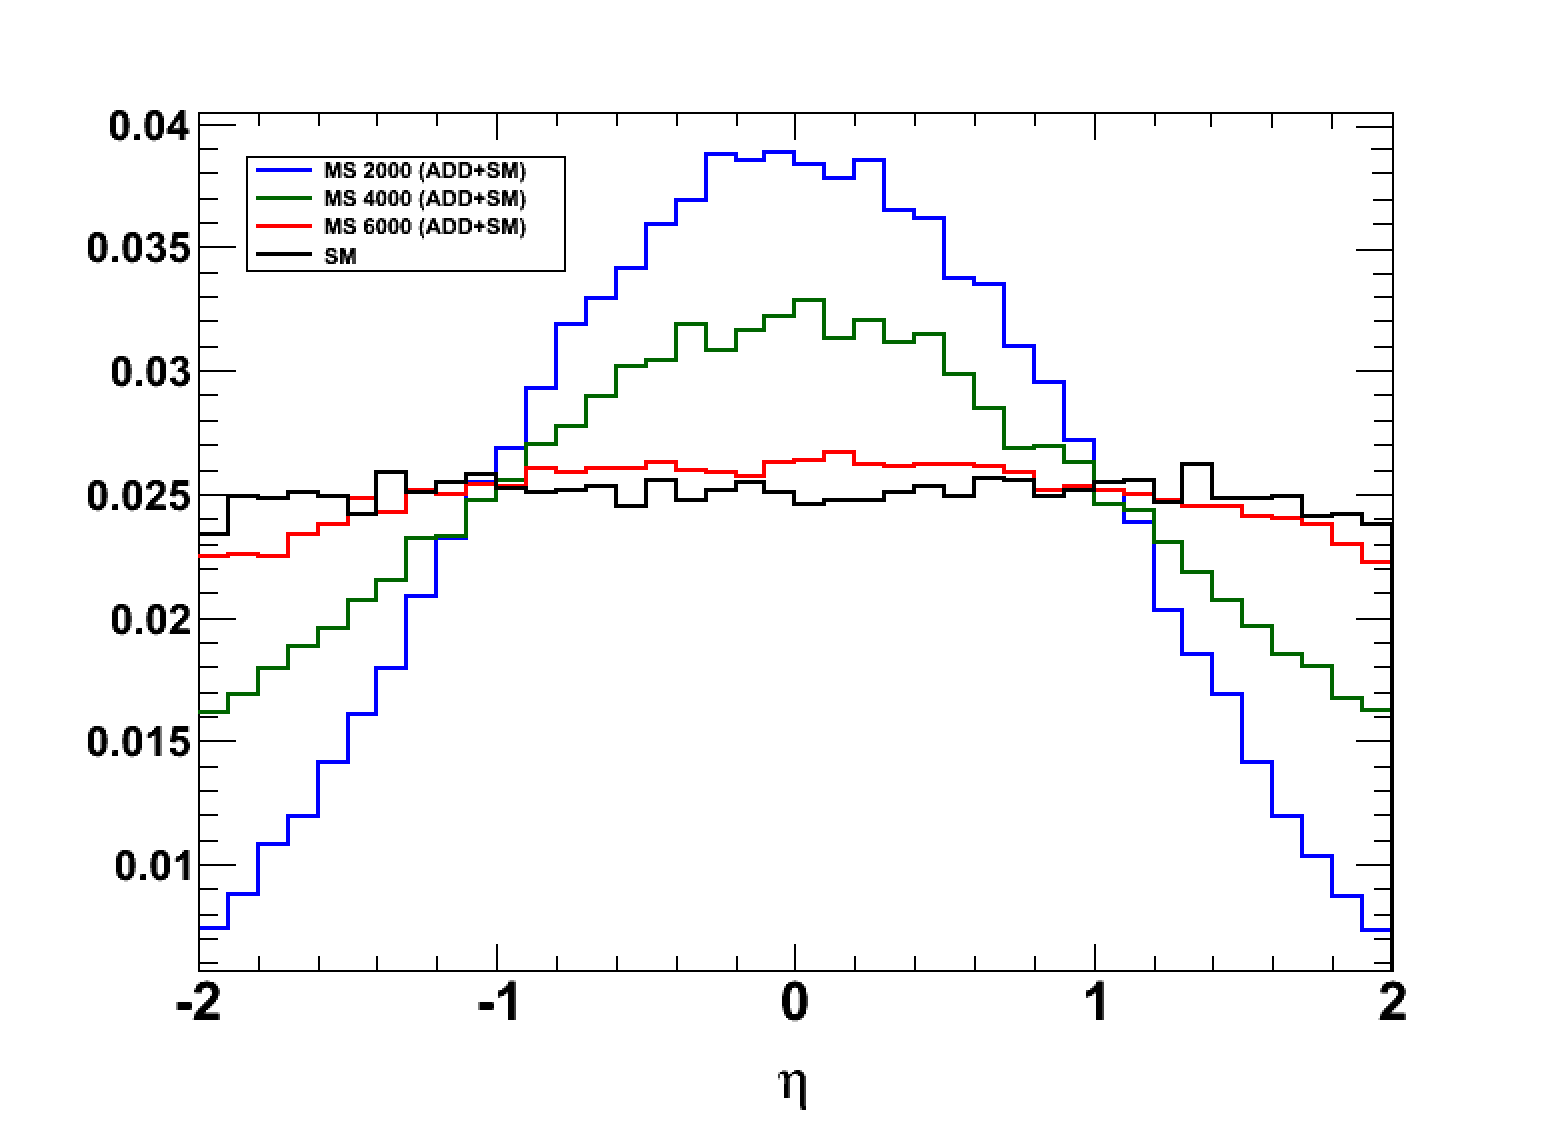
\includegraphics[width=0.75\textwidth]{figures/add_signal_with_sm_photon_eta_edit.png}
  \caption{Combined ADD\texttt{+}SM signal distributions in photon $\eta$ compared again the corresponding SM background distribution.}
  \label{fig:ADD_photon_eta}
\end{figure}

In general, the diphoton invariant mass distributions from different conventions are expected to differ. For example, Fig.~\ref{fig:Hewett_pos_neg} compares the distributions between Hewett\texttt{+} and Hewett\texttt{-} using $\Ms=4000\GeV$. The negative interference gives rise to a pronounced valley in the distribution. Fig.~\ref{fig:HLZ_vary_nED} shows a comparison of the invariant mass distributions within the HLZ convention using $\Ms=2500\GeV$ for different values of \nED. The shape of the distribution using $\nED=2$ differs from the others due to the different form of $\mathcal{F}$ as shown in Eq.~(\ref{eqn:add_f_conventions}). The distributions for $\nED>2$ are more signal like for lower values of \nED and become more background-like at higher values.

 \begin{figure}[!htbp]
  \centering
  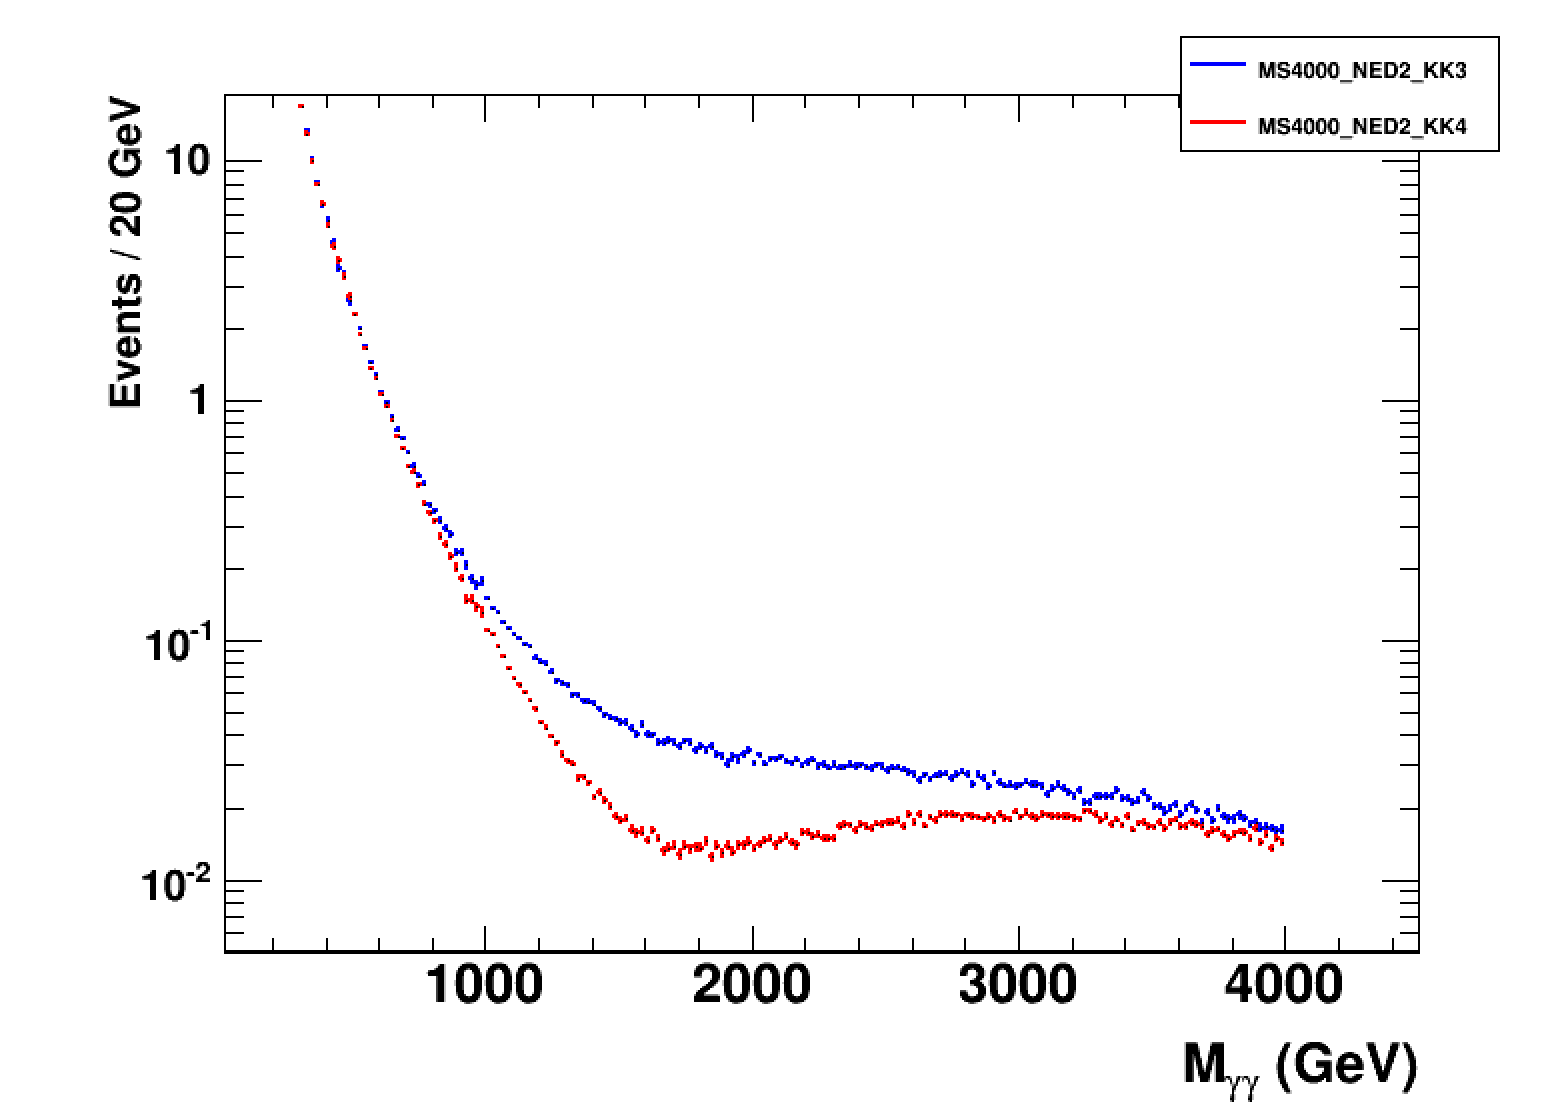
\includegraphics[width=0.75\textwidth]{figures/Hewett_pos_vs_neg}
  \caption{Comparison of the \Mgg spectra between the Hewett\texttt{+} (blue) and Hewett\texttt{-} (red) conventions using $\Ms=4000\GeV$.}
  \label{fig:Hewett_pos_neg}
\end{figure}

 \begin{figure}[!htbp]
  \centering
  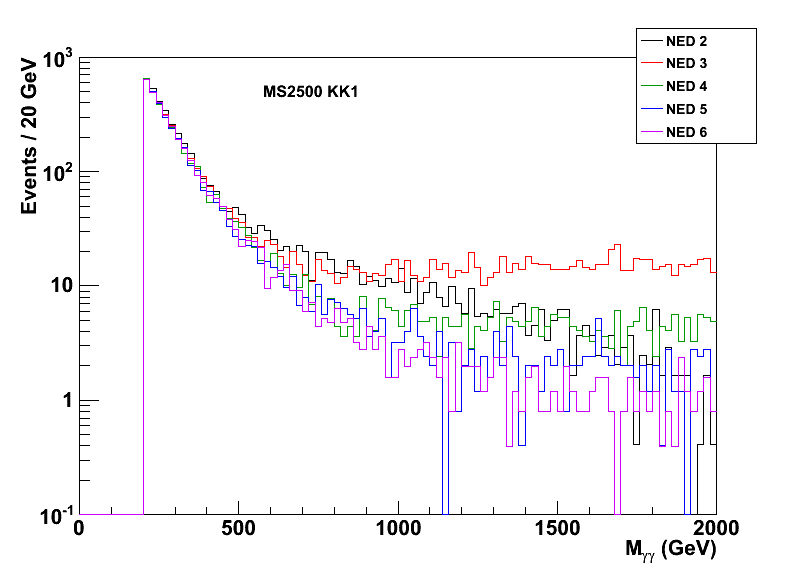
\includegraphics[width=0.75\textwidth]{figures/DiPhoton_Minv_MS2500_KK1_plot}
  \caption{The \Mgg spectra for different signals from the HLZ convention using $\Ms=2500\GeV$ for different values of \nED.}
  \label{fig:HLZ_vary_nED}
\end{figure}

In some cases, the parameter $\mathcal{F}$ is the same between different conventions. This can be observed from Eq.~(\ref{eqn:add_f_conventions}) and allows for a relation among different conventions. For example, the value of $\mathcal{F}$ using the HLZ convention with $\nED=4$ equals that of GRW, so these two conventions should be equivalent. This is demonstrated in Fig.~\ref{fig:ADD_cross_checks} (left) by comparing the diphoton invariant mass distributions from each convention. Notice the value of \etaG is the same for both signals. In addition, the GRW and Hewett conventions do not depend on \nED. We verify that this is in fact the case in the \SHERPA implementation by comparing the \Mgg spectra using GRW with $\nED = 2$ and $\nED = 4$ in Fig.~\ref{fig:ADD_cross_checks} (right).

\begin{figure}[!htbp]
  %\centering
  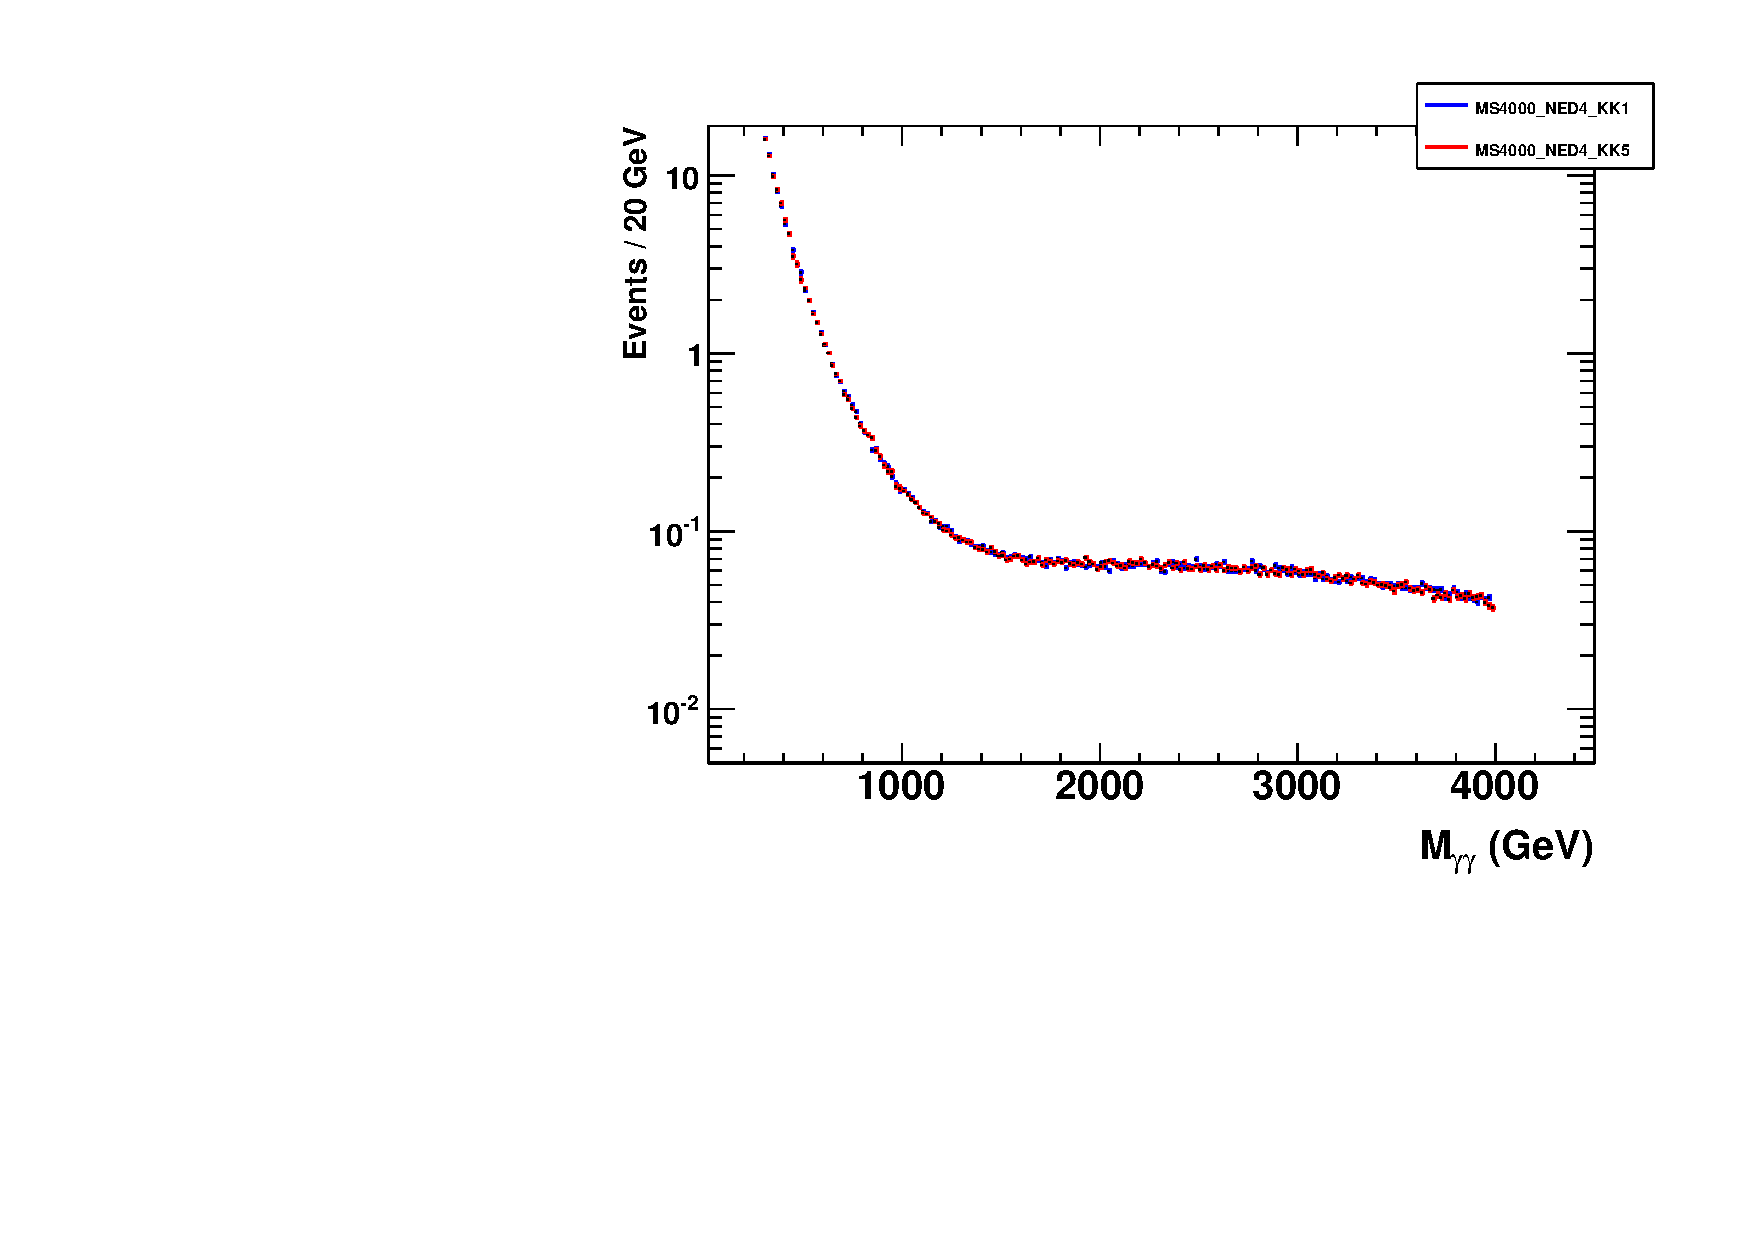
\includegraphics[width=0.50\textwidth]{figures/diphoton_mgg_acc_MS4000_NED4_KK1_MS4000_NED4_KK5}
  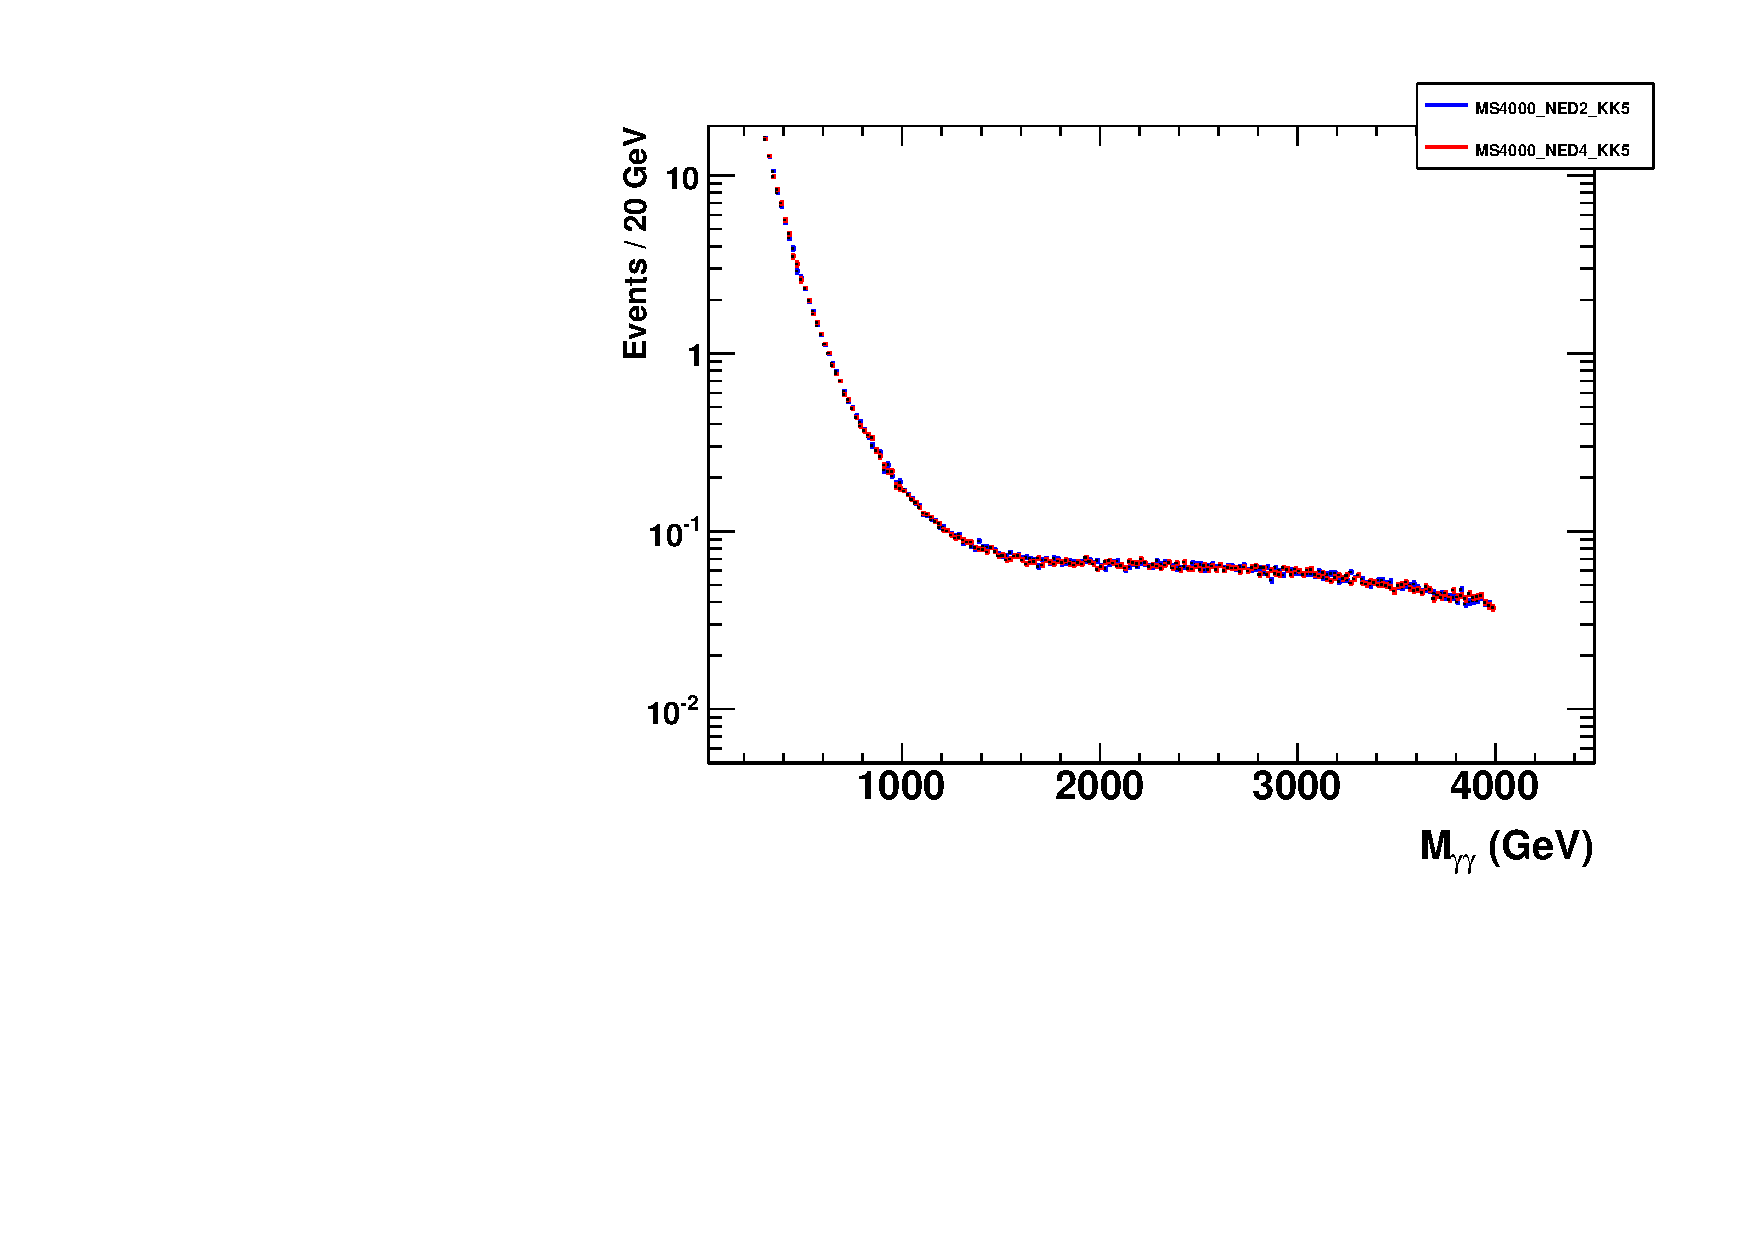
\includegraphics[width=0.50\textwidth]{figures/diphoton_mgg_acc_MS4000_NED2_KK5_MS4000_NED4_KK5}
  \caption{The \mgg distributions demonstrating that the HLZ convention using $\nED = 4$ (blue) is equivalent to the GRW convention (red), both for $\Ms = 4000\GeV$ (right), and those from the GRW convention using $\Ms = 4000\GeV$ for $\nED = 2$ (blue) and 4 (red), demonstrating the equivalence of different \nED values (left).}
  \label{fig:ADD_cross_checks}
\end{figure}

Other conventions can be related to each other through the \etaG parameter. This is because the diphoton invariant mass distributions from different conventions are equivalent if they have the same value of \etaG. Essentially this means an ADD model point with a particular \Ms value in one convention produces the same physical diphoton invariant mass distribution as a specific model point using a different \Ms value in another convention; the precise points which will have equivalent spectra are ones which share the same value for \etaG. For example, the diphoton spectrum obtained using the Hewett\texttt{+} convention with $\Ms=4000\GeV$ is equivalent to the spectrum obtained for the GRW convention but with $\Ms=4478\GeV$, as illustrated in Fig.~\ref{fig:ADD_diff_convention_equiv} (left). Using \etaG, this arises through the relation $M_{\mathrm{S}}^{\rm GRW} = (\pi/2)^{1/4} M_{\mathrm{S}}^{\rm Hewett\texttt{+}}$. Similarly, we can relate the HLZ conventions for $\nED > 2$ among each other. (The $\mathcal{F}$ parameter for HLZ with $\nED=2$ involves $\hat{s}$ and cannot be related to the other conventions.) For example, the HLZ convention with $\nED = 6$ is related to the HLZ convention using $\nED = 3$ through the \etaG parameter by $M_{\mathrm{S}}^{\rm{HLZ} \,(\nED=3)} = 4^{1/4} M_{\mathrm{S}}^{\rm{HLZ} \,(\nED=6)}$. Therefore, the diphoton invariant mass distributions from the HLZ convention with $\nED = 6$ using $\Ms = 4000\GeV$ and the HLZ convention with $\nED = 3$ using $\Ms = 5657\GeV$ are equivalent, as shown in Fig.~\ref{fig:ADD_diff_convention_equiv} (right).

\begin{figure}[!htbp]
  \centering
  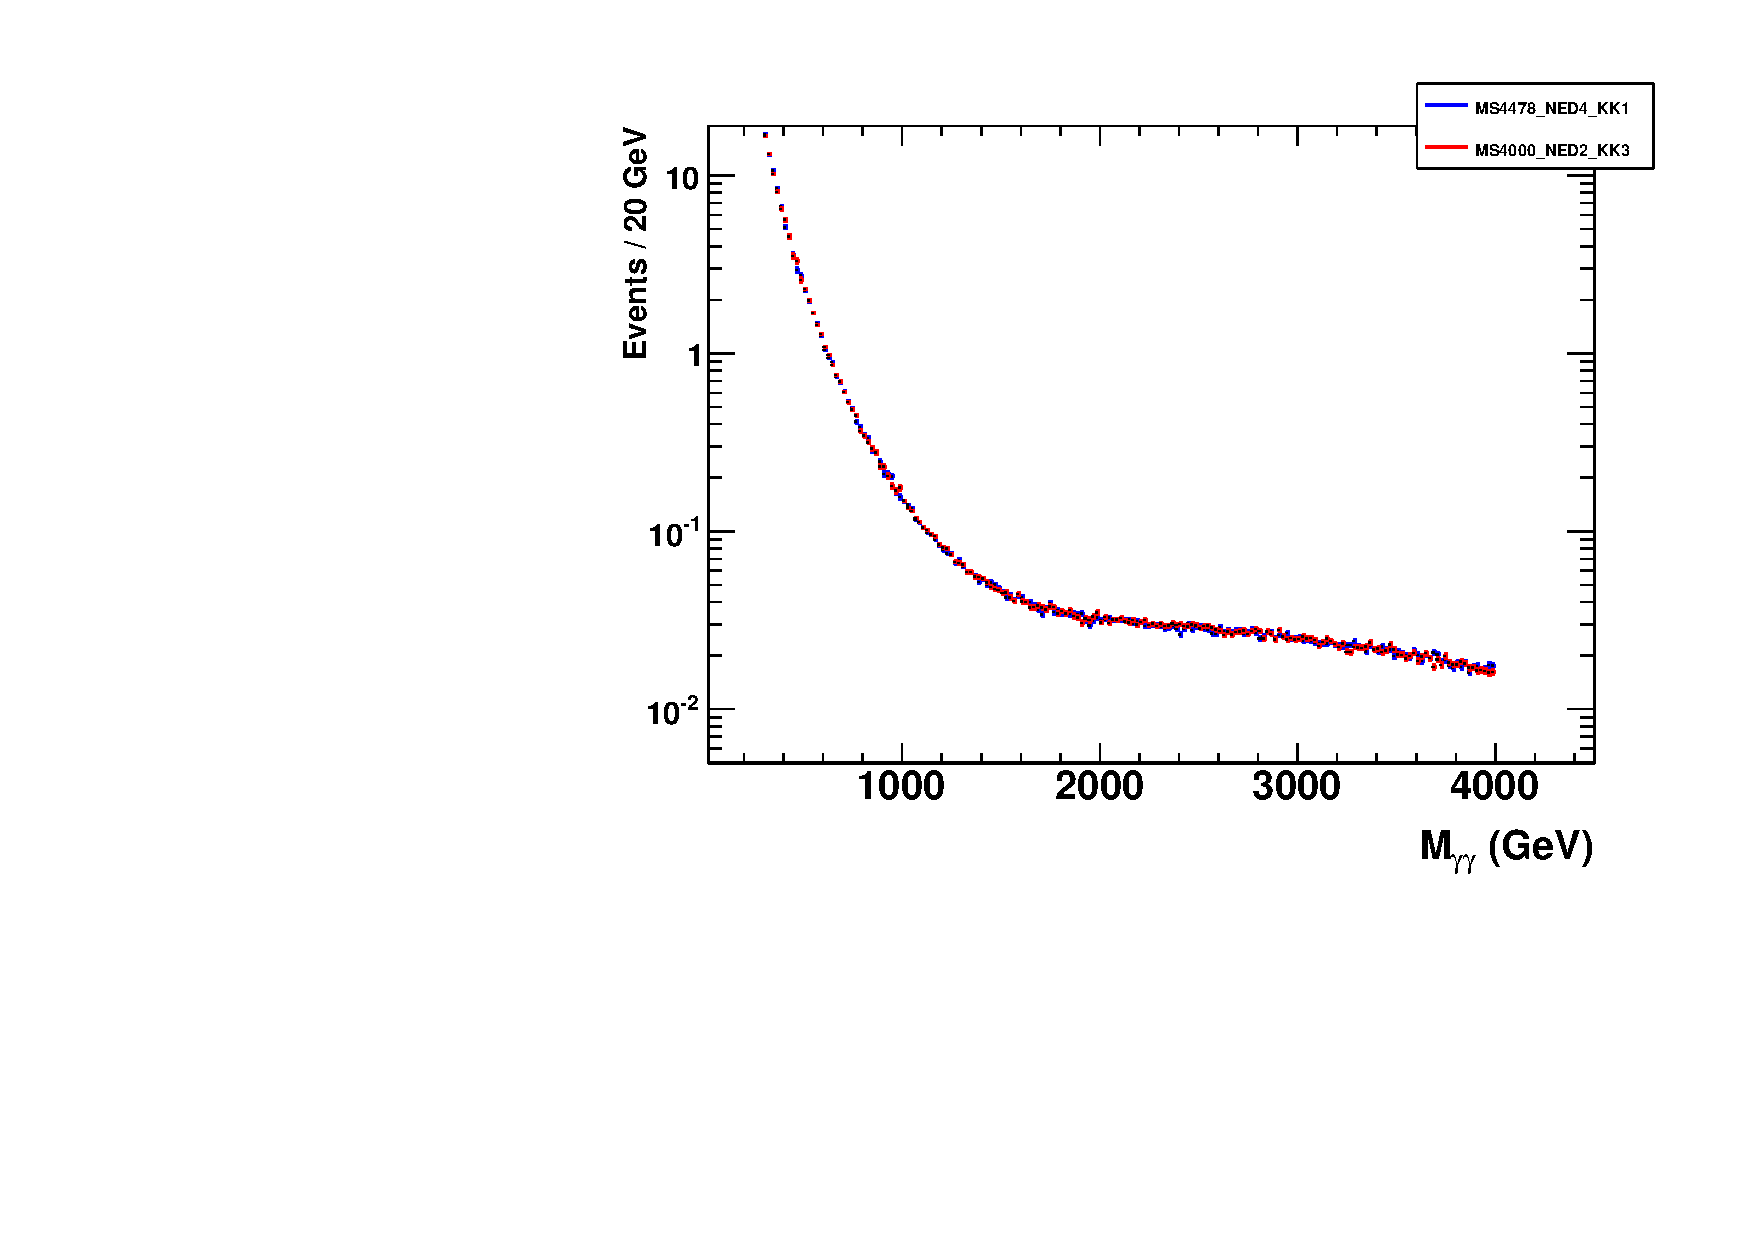
\includegraphics[width=0.51\textwidth]{figures/diphoton_mgg_acc_MS4478_NED4_KK1_MS4000_NED2_KK3.pdf}
  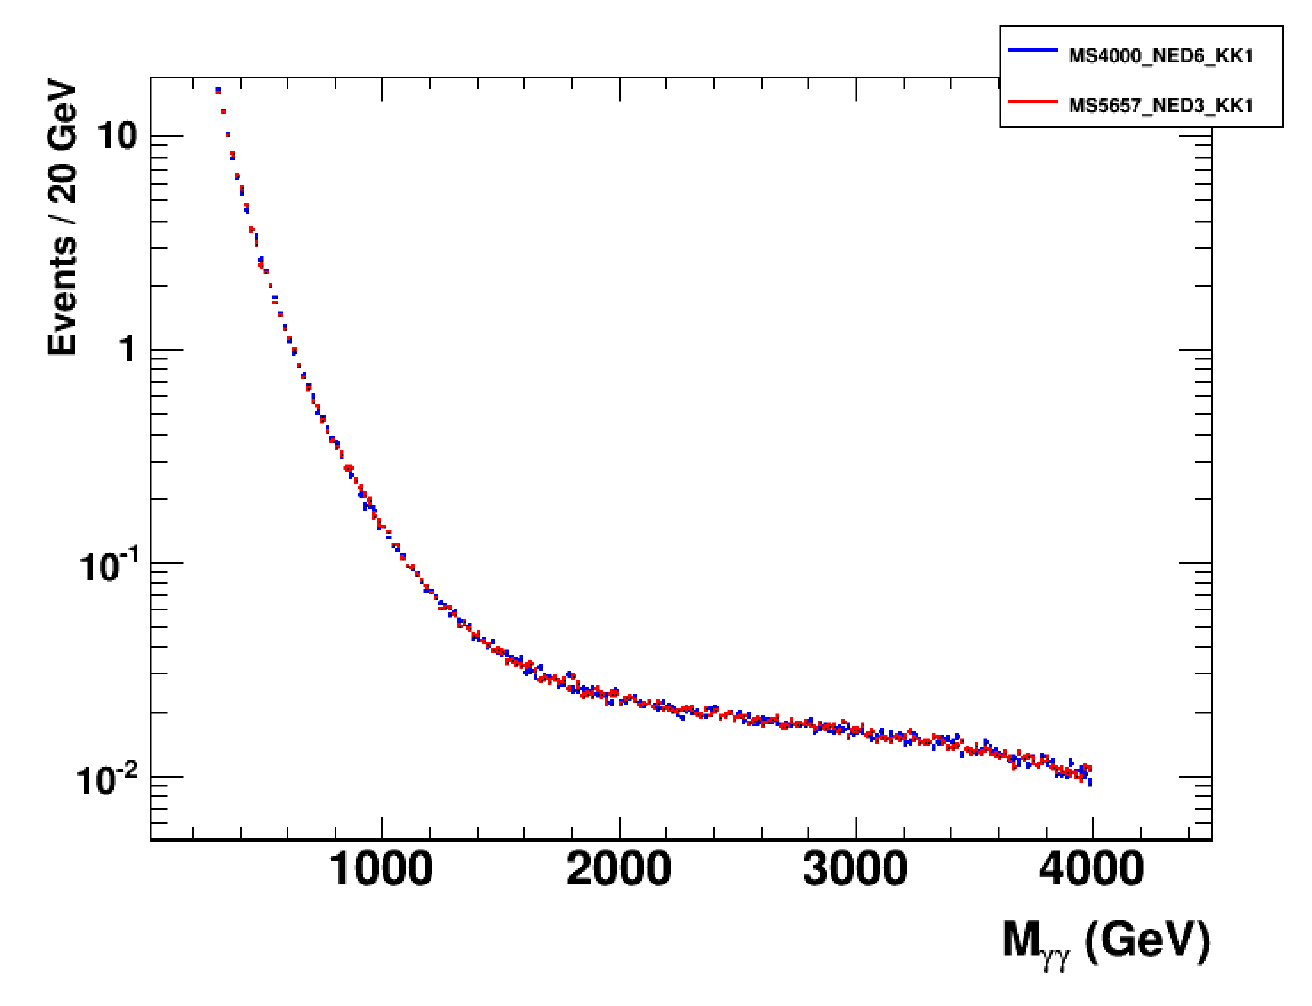
\includegraphics[width=0.4650\textwidth]{figures/HLZ_etaG_scaling.png}
  \caption{The \mgg distributions for the Hewett\texttt{+} convention (red) using $\Ms = 4000\GeV$ and the GRW convention (blue) using $\Ms = 4478\GeV$ (left). The \mgg distributions for the HLZ convention (blue) using $\nED = 6$ with $\Ms = 4000\GeV$ and for the HLZ convention (red) using $\nED=3$ with $\Ms = 5657\GeV$ (right). In each plot, the two conventions have the same value of \etaG and their spectra are shown to be equivalent.}
  \label{fig:ADD_diff_convention_equiv}
\end{figure}


\section{Signal Samples}

For this analysis, we consider the ADD parameter space spanning $\Ms = 3$, 3.5, 4, \dots, 6, 7, \dots, 11\TeV for each of the following conventions: GRW; HLZ assuming $\nED=2$, 3, \dots, 7; Hewett\texttt{+}; and Hewett\texttt{-}. However, the equivalence of signal points demonstrated using the \etaG parameterization allows us to significantly reduce the number of MC samples required to span this space for signal generation. Instead of generating all these convention possibilities, consistent with Eq.~(\ref{eqn:add_f_conventions}), we only need to generate events for the following conventions:
\begin{itemize}
	\item HLZ ($\KK=1$) assuming $\nED = 4$, which has constant positive interference; 
	\item HLZ ($\KK=1$) assuming $\nED = 2$, which has positive interference with $\hat{s}$ dependence;
	\item Hewett\texttt{-} ($\KK=4$), which has negative interference. 
\end{itemize}
All other conventions listed above have constant positive interference and can be inferred from the samples generated using HLZ assuming $\nED = 4$. The negative interference and $\hat{s}$ dependence among the conventions needs to be treated separately.

Each of these three conventions requires a separate MC sample for each value of \Ms. The example \SHERPA run card in Appendix~\ref{ch:ADD_run_card} shows the configuration for HLZ with $\nED=4$ using $\Ms=3500\GeV$. However, to improve the statistics for sampling the phase space, each sample is broken into several diphoton invariant mass \Mgg bins. The bin ranges depend on the particular choice of parameters but are typically 200-500, 500-1000, 1000-2000, 2000-4000, and 4000-\Ms\GeVns, where the last bin is cut off at $\Mgg=\Ms$. Further restrictions are imposed on the phase space for each sample: the kinematic selections requiring photon $\pt > 70\GeV$ and photon $|\eta| < 2.8$. The MC samples are generated for pp collisions at $\sqrt{s}=13\TeV$. The interactions of the generated particles with the CMS detector are simulated using \GEANTfour, which includes the effects of pileup.

Each sample is prepared and validated privately before internal requests within the CMS Collaboration are submitted for production of the fully simulated samples using the 2016 CMS detector conditions approved for collaboration-wide use. An example, internal dataset path for the MC sample corresponding to the model point for HLZ with $\nED=4$ using $\Ms=3500\GeV$ in the bin $\Mgg=2000$-3000\GeV has the form \texttt{/ADDGravToGG\_\allowbreak MS-3500\_\allowbreak NED-4\_\allowbreak KK-1\_\allowbreak M-2000To3000\_\allowbreak 13TeV-\allowbreak sherpa/\allowbreak RunIISummer16MiniAODv2-\allowbreak PUMoriond17\_\allowbreak 80X\_\allowbreak mcRun2\_\\\allowbreak asymptotic\_\allowbreak 2016\_\allowbreak TrancheIV\_\allowbreak v6/\allowbreak MINIAODSIM}. Of its three parts, the first specifies the model point, the second indicates the internal MC campaign used to reproduce the 2016 CMS detector conditions, and the final part signifies the custom data format used within the collaboration. Each sample contains 100,000 fully simulated events. Table~\ref{tab:ADD_signal_samples} provides a summary of all the generated ADD samples and their associated cross sections. In total, 122 ADD samples were produced totaling 12,200,000 events.

\begin{table}[htbp!]
	\centering
	\caption{Cross sections (in units of fb) for the combined ADD\texttt{+}SM samples used in the analysis. For $\Ms=3$-$4\TeV$, the last \Mgg bin is from 2-\Ms\TeVns, i.e., there is no bin splitting into 2-$X\TeV$ and $X$-\Ms\TeVns. For $\Ms=4.5$ or 5\TeV, the bin edge is at $X = 3\TeV$. For $\Ms>5\TeV$, $X=4\TeV$.}
	\label{tab:ADD_signal_samples}
  \vspace{\baselineskip}
	\begin{tabular}{ll|ccccc}
		\hline % total samples 7+31*3+22 = 122
		\hline % requested: 82+40 = 122
		\Ms ({\TeVns}) & \KK convention & 0.2-0.5\TeV & 0.5-1\TeV & 1-2\TeV  & 2-$X\TeV$ & $X$-\Ms\TeVns \\
		\hline
		3          & HLZ ($\nED=2$) & -            & 139.7      & 91.39     & 11.6       & -            \\
		           & HLZ ($\nED=4$) & 898.5        & 89.66      & 51.64     & 55.18      & -            \\
		           & Hewett\texttt{-}        & -            & 73.31      & 17.52     & 20.2       & -            \\
		3.5        & HLZ ($\nED=2$) & -            & 102.6      & 45.1      & 9.442      & -            \\
		           & HLZ ($\nED=4$) & 892.4        & 81.04      & 21.26     & 23.65      & -            \\
		           & Hewett\texttt{-}        & -            & 73.98      & 8.453     & 8.239      & -            \\
		4          & HLZ ($\nED=2$) & -            & 89.81      & 25.53     & 6.604      & -            \\
		           & HLZ ($\nED=4$) & 889.4        & 78.21      & 12.34     & 10.5       & -            \\
		           & Hewett\texttt{-}        & -            & 74.27      & 6.494     & 3.474      & -            \\
		4.5        & HLZ ($\nED=2$) & -            & 83.73      & 16.61     & 3.809      & 0.6004       \\
		           & HLZ ($\nED=4$) & 896.6        & 77.03      & 9.129     & 2.688      & 2.27         \\
		           & Hewett\texttt{-}        & -            & 74.85      & 6.033     & 0.7721     & 0.7878       \\
		5          & HLZ ($\nED=2$) & -            & 80.25      & 12.21     & 2.423      & 0.5167       \\
		           & HLZ ($\nED=4$) & 894          & 76.4       & 7.829     & 1.382      & 1.193        \\
		           & Hewett\texttt{-}        & -            & 74.71      & 5.999     & 0.3925     & 0.3902       \\
		5.5        & HLZ ($\nED=2$) & -            & 79.11      & 9.948     & 1.969      & 0.04542      \\
		           & HLZ ($\nED=4$) & 894.7        & 75.99      & 7.209     & 1.218      & 0.2419       \\
		           & Hewett\texttt{-}        & -            & 75.22      & 6.047     & 0.3688     & 0.08207      \\
		6          & HLZ ($\nED=2$) & -            & 78.19      & 8.717     & 1.382      & 0.0446       \\
		           & HLZ ($\nED=4$) & 900.4        & 75.98      & 6.887     & 0.7727     & 0.1393       \\
		           & Hewett\texttt{-}        & -            & 75.35      & 6.09      & 0.264      & 0.04472      \\
		7          & HLZ ($\nED=2$) & -            & 77.18      & 7.501     & 0.7842     & 0.03281      \\
		           & HLZ ($\nED=4$) & -            & 76.39      & 6.598     & 0.4351     & 0.04842      \\
		8          & HLZ ($\nED=2$) & -            & 76.27      & 6.941     & 0.5179     & 0.0214       \\
		           & HLZ ($\nED=4$) & -            & 76.23      & 6.437     & 0.3247     & 0.01974      \\
		9          & HLZ ($\nED=2$) & -            & 76.27      & 6.734     & 0.3959     & 0.01394      \\
		           & HLZ ($\nED=4$) & -            & 75.69      & 6.386     & 0.2802     & 0.009672     \\
		10         & HLZ ($\nED=2$) & -            & 76.08      & 6.554     & 0.3313     & 0.009366     \\
		           & HLZ ($\nED=4$) & -            & 75.89      & 6.377     & 0.259      & 0.005716     \\
		11         & HLZ ($\nED=2$) & -            & 75.97      & 6.527     & 0.2997     & 0.006698     \\
		           & HLZ ($\nED=4$) & -            & 75.59      & 6.361     & 0.2504     & 0.003906     \\
		\hline
		\hline
	\end{tabular}
\end{table}

The LO SM background samples and cross sections used with the above LO ADD\texttt{+}SM samples are tabulated in Table~\ref{tab:signal_samples_background}. Like the ADD\texttt{+}SM samples, these are produced in \Mgg bins resulting in 6 samples each of 100,000 events. Only the first part of the CMS dataset path is listed as the second and third parts are the same as above. Appendix~\ref{ch:LO_SM_run_card} shows an example \SHERPA run card used to generate this background.

\begin{table}[htbp!]
	\caption{The LO SM background MC samples. The full, internal CMS path name is specified by appending the dataset path with \texttt{/RunIISummer16MiniAODv2-\allowbreak PUMoriond17\_\allowbreak 80X\_\allowbreak mcRun2\_\allowbreak asymptotic\_\allowbreak 2016\_\allowbreak TrancheIV\_\allowbreak v6/\allowbreak MINIAODSIM}}
	\label{tab:signal_samples_background}
	\centering
  \vspace{\baselineskip}
	\begin{tabular}{lc}
	\hline \hline
	Dataset path & Cross section (pb) \\
	\hline
	/GG\_M-200To500\_Pt-70\_13TeV-sherpa    & 8.923e-01 \\
	/GG\_M-500To1000\_Pt-70\_13TeV-sherpa   & 7.592e-02 \\
	/GG\_M-1000To2000\_Pt-70\_13TeV-sherpa  & 6.292e-03 \\
	/GG\_M-2000To4000\_Pt-70\_13TeV-sherpa  & 2.315e-04 \\
	/GG\_M-4000To8000\_Pt-70\_13TeV-sherpa  & 1.669e-06 \\
	/GG\_M-8000To13000\_Pt-70\_13TeV-sherpa & 5.430e-11 \\
	\hline \hline
	\end{tabular}
\end{table}

 The diphoton invariant mass distributions for the three \KK conventions considered in this analysis using $\Ms=3$, 3.5, 4, \dots, 6\TeV are shown in Fig.~\ref{fig:signal} (left). Notice the spectra are truncated at their corresponding value of \Ms. After subtraction of the SM background, the resulting \mgg distributions are shown in Fig.~\ref{fig:signal} (right), for each of these three \KK conventions. These are the final \mgg distributions containing only the ADD signal and interference between the ADD signal and the SM background. Similar distributions are shown in Fig.~\ref{fig:signal_high_Ms} for the higher values of $\Ms = 6$, 7, 8, 9, and 10\TeV using HLZ assuming $\nED=4$ compared against the distribution from HLZ with $\nED = 2$ and $\Ms = 8\TeV$, shown in the EBEB and EBEE categories. For these values of \Ms, the low-mass region remains dominated by the SM background, while the high-mass region is signal dominated.

These SM background-subtracted ADD signal distributions represent the additional effect of the large extra-dimensional signal and are used in the limit setting procedure, as described in Section~\ref{sec:limit_setting}.

\begin{figure}[tbp!]
  \centering
	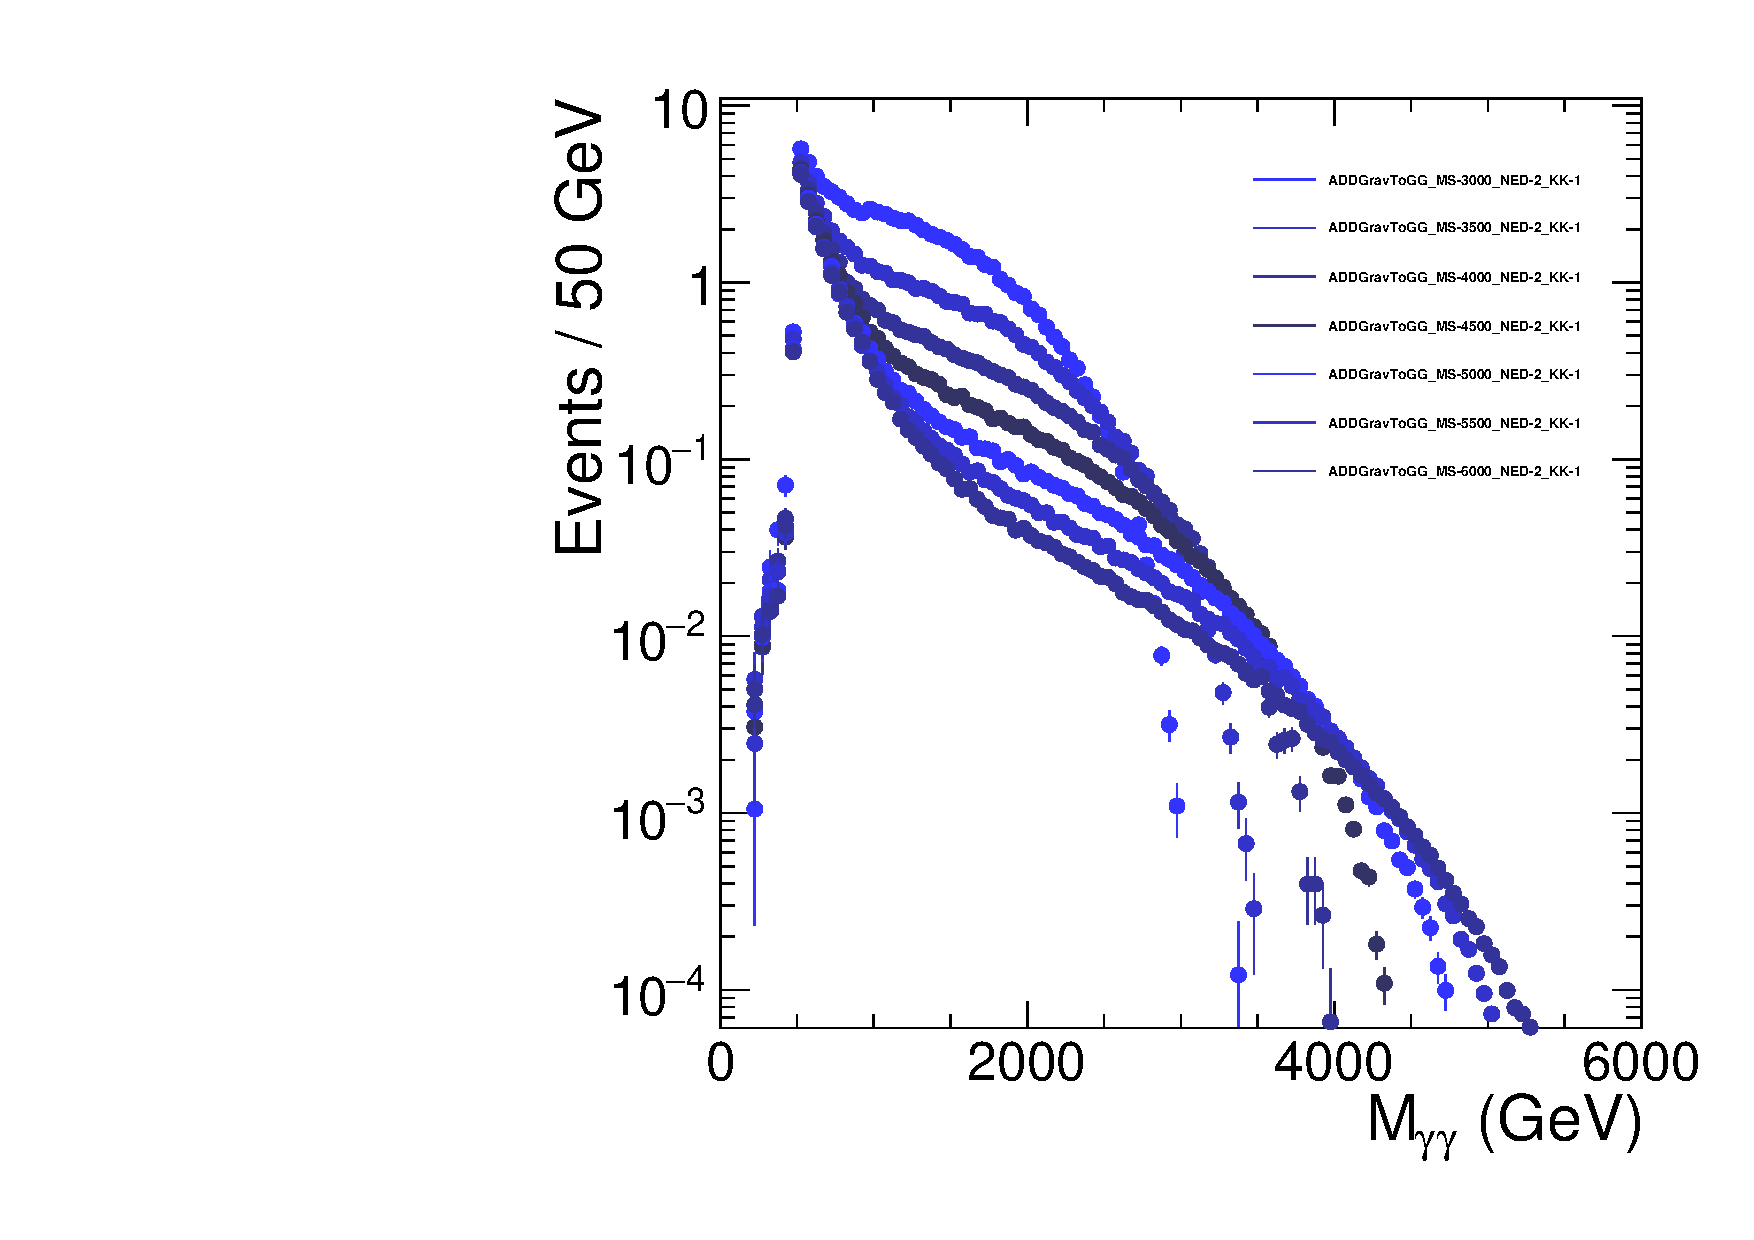
\includegraphics[angle=0,width=0.41\textwidth]{figures/ADDGravToGG_NED-2_KK-1.pdf}
	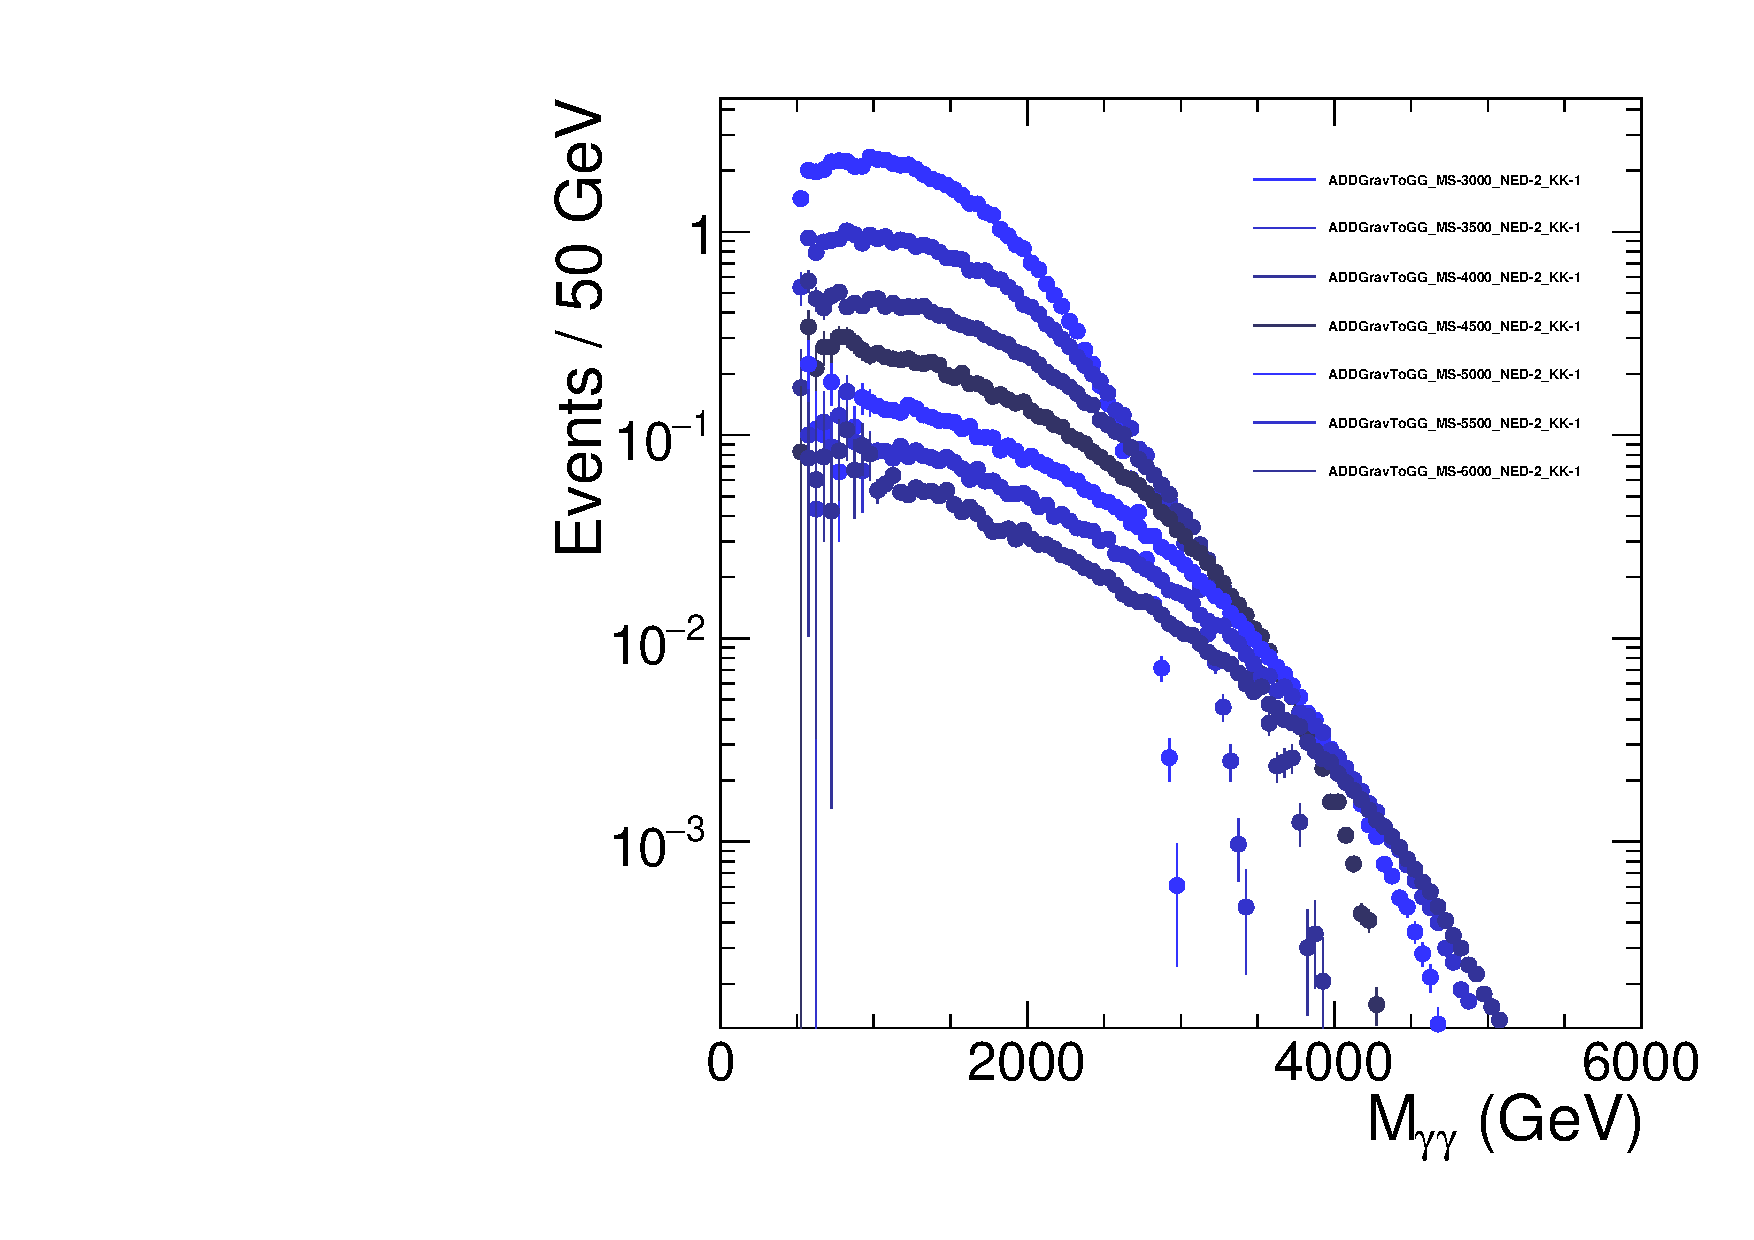
\includegraphics[angle=0,width=0.41\textwidth]{figures/ADDGravToGG_NED-2_KK-1_bkg_sub.pdf}
	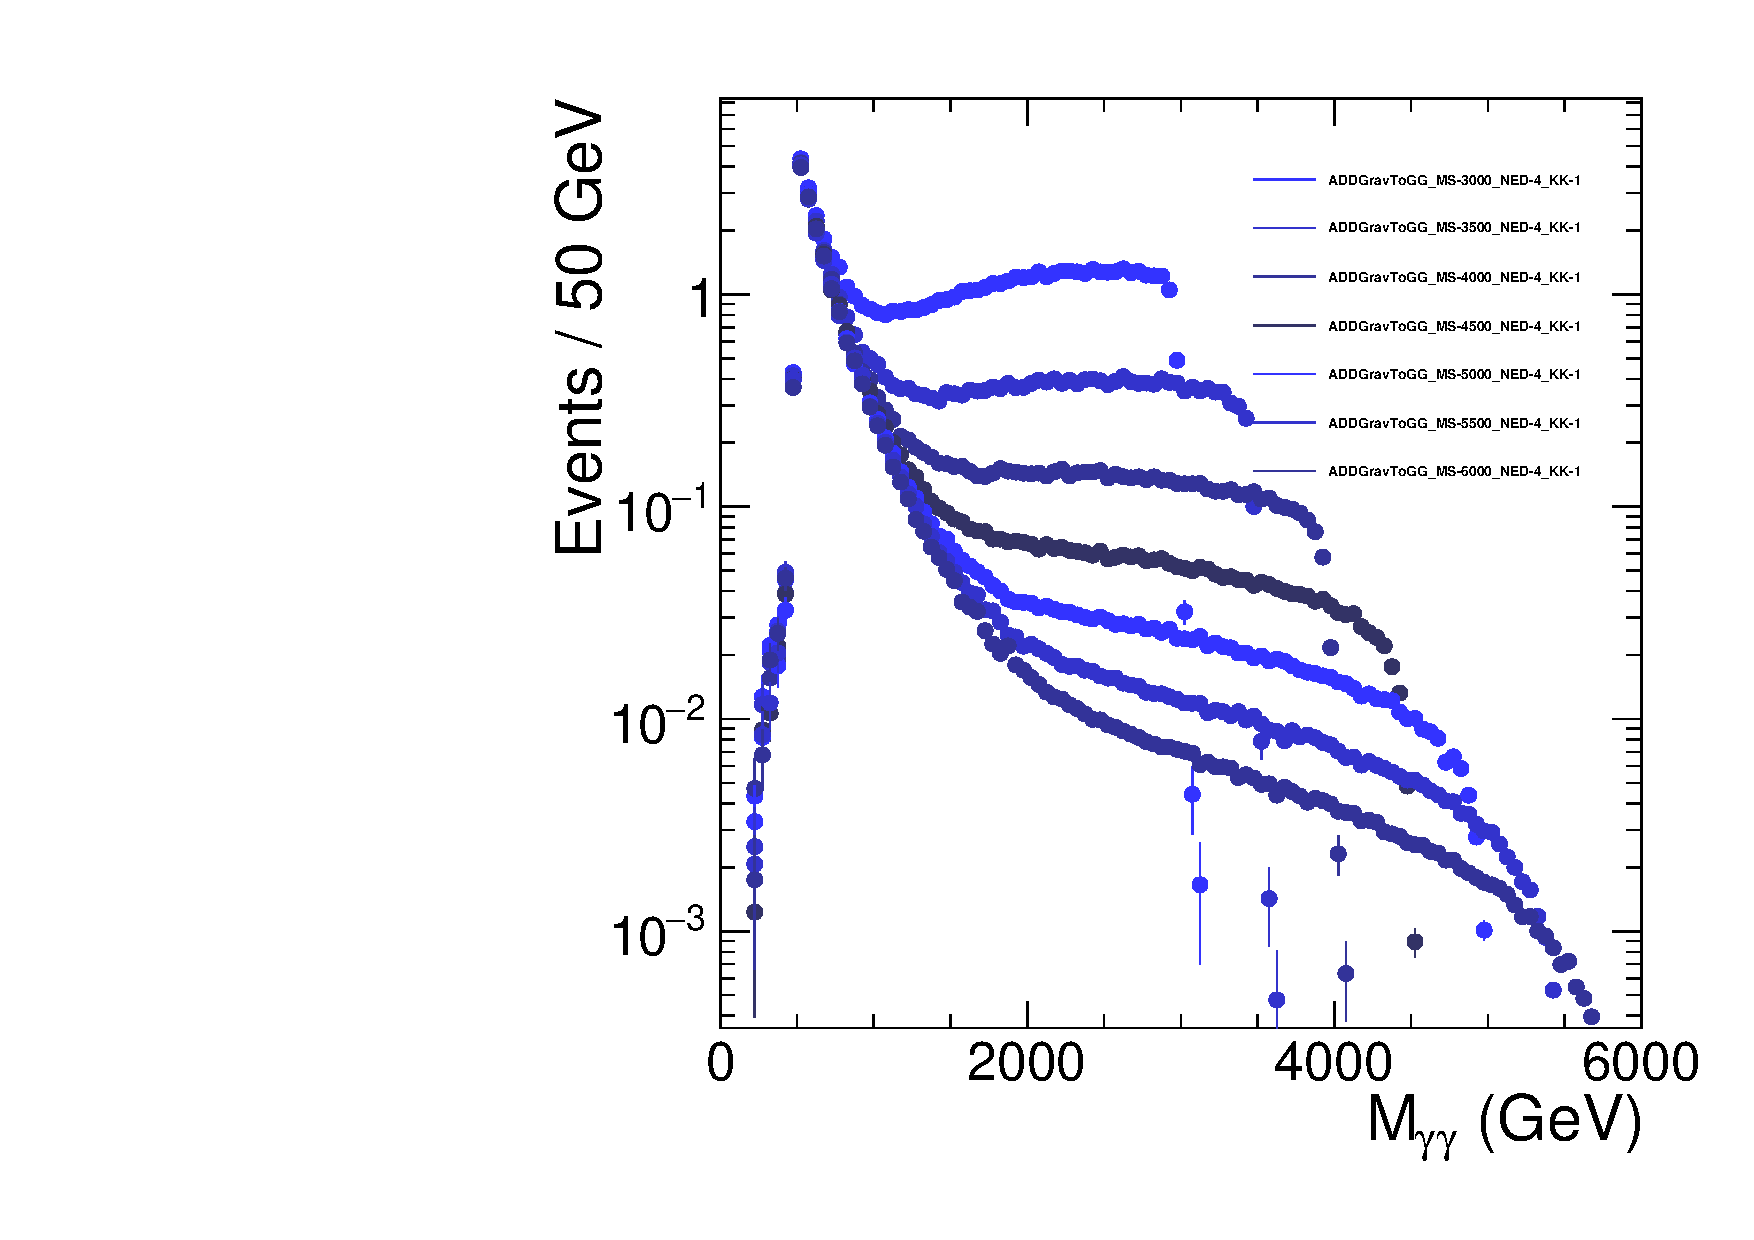
\includegraphics[angle=0,width=0.41\textwidth]{figures/ADDGravToGG_NED-4_KK-1.pdf}
	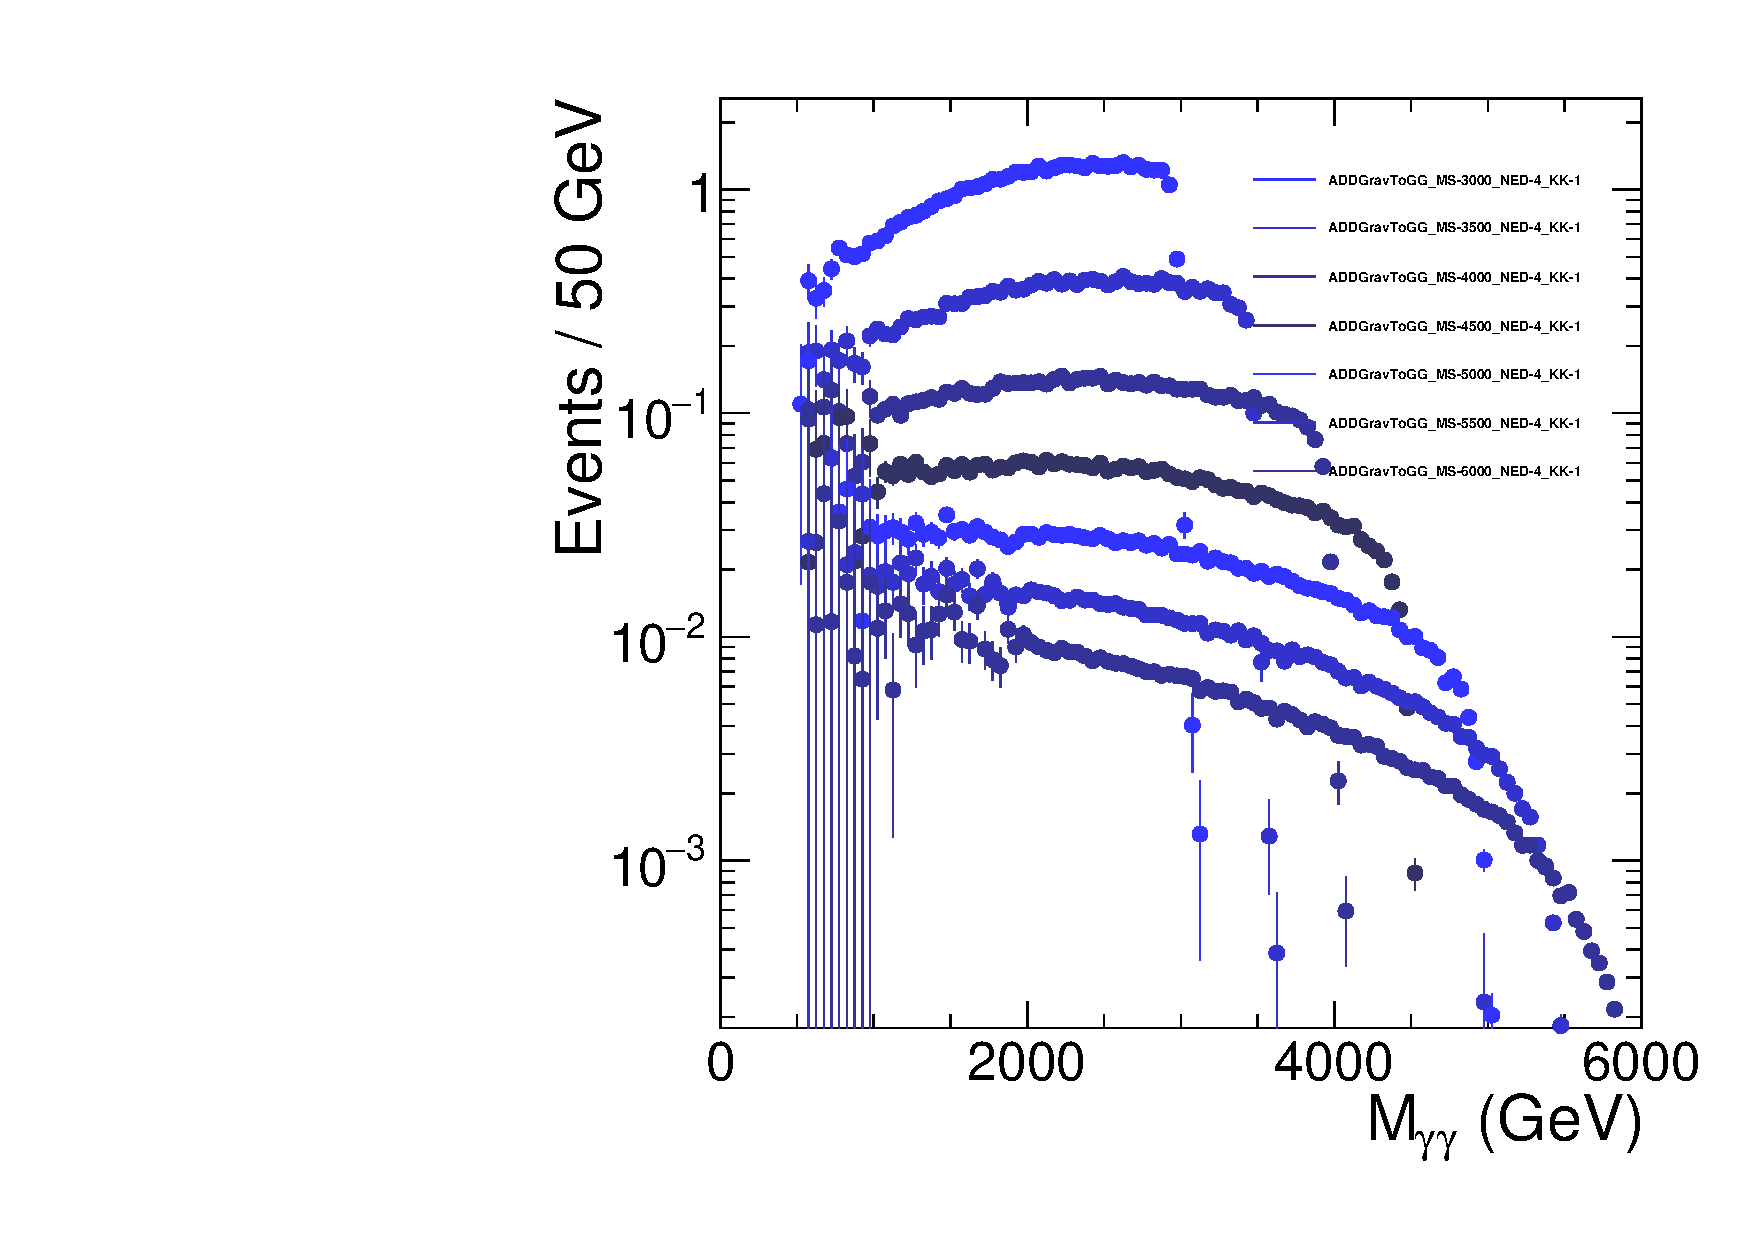
\includegraphics[angle=0,width=0.41\textwidth]{figures/ADDGravToGG_NED-4_KK-1_bkg_sub.pdf}
	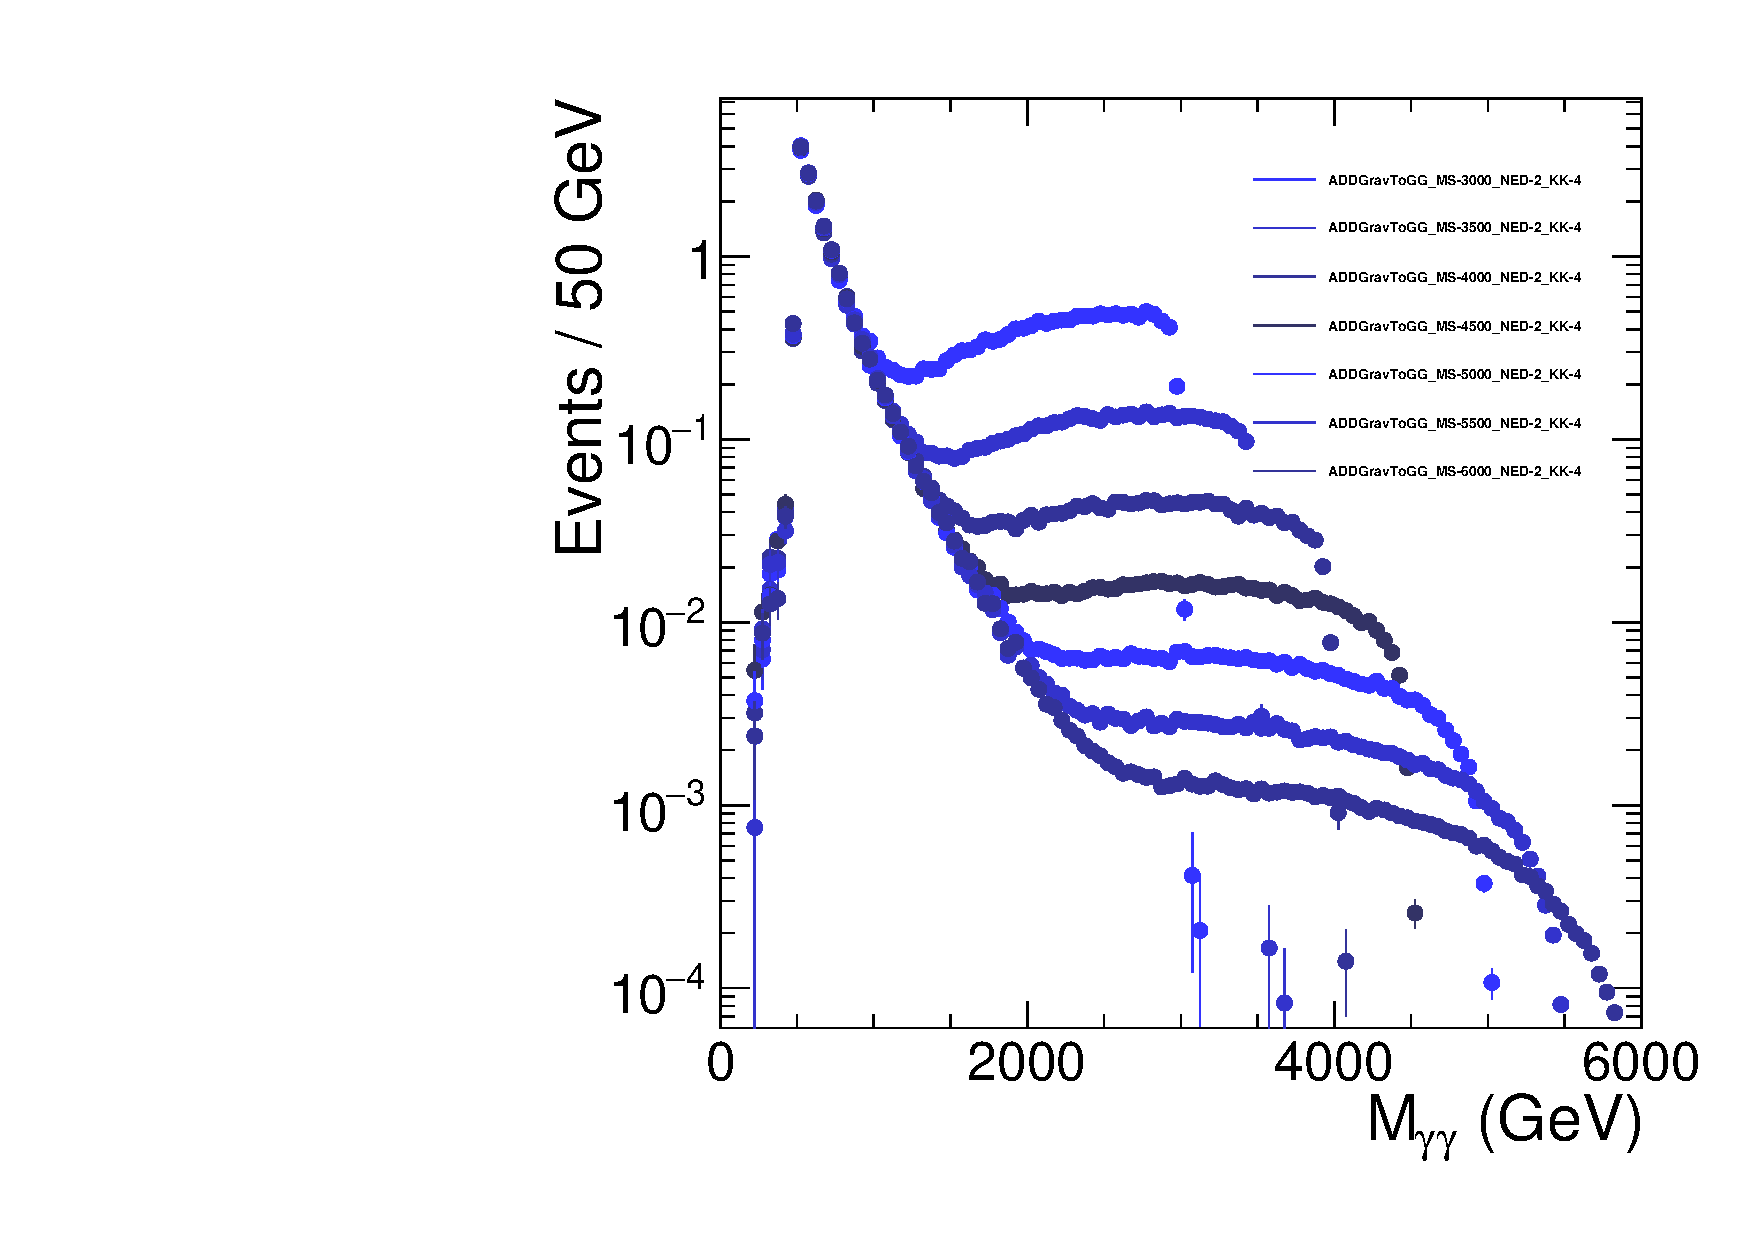
\includegraphics[angle=0,width=0.41\textwidth]{figures/ADDGravToGG_NED-2_KK-4.pdf}
	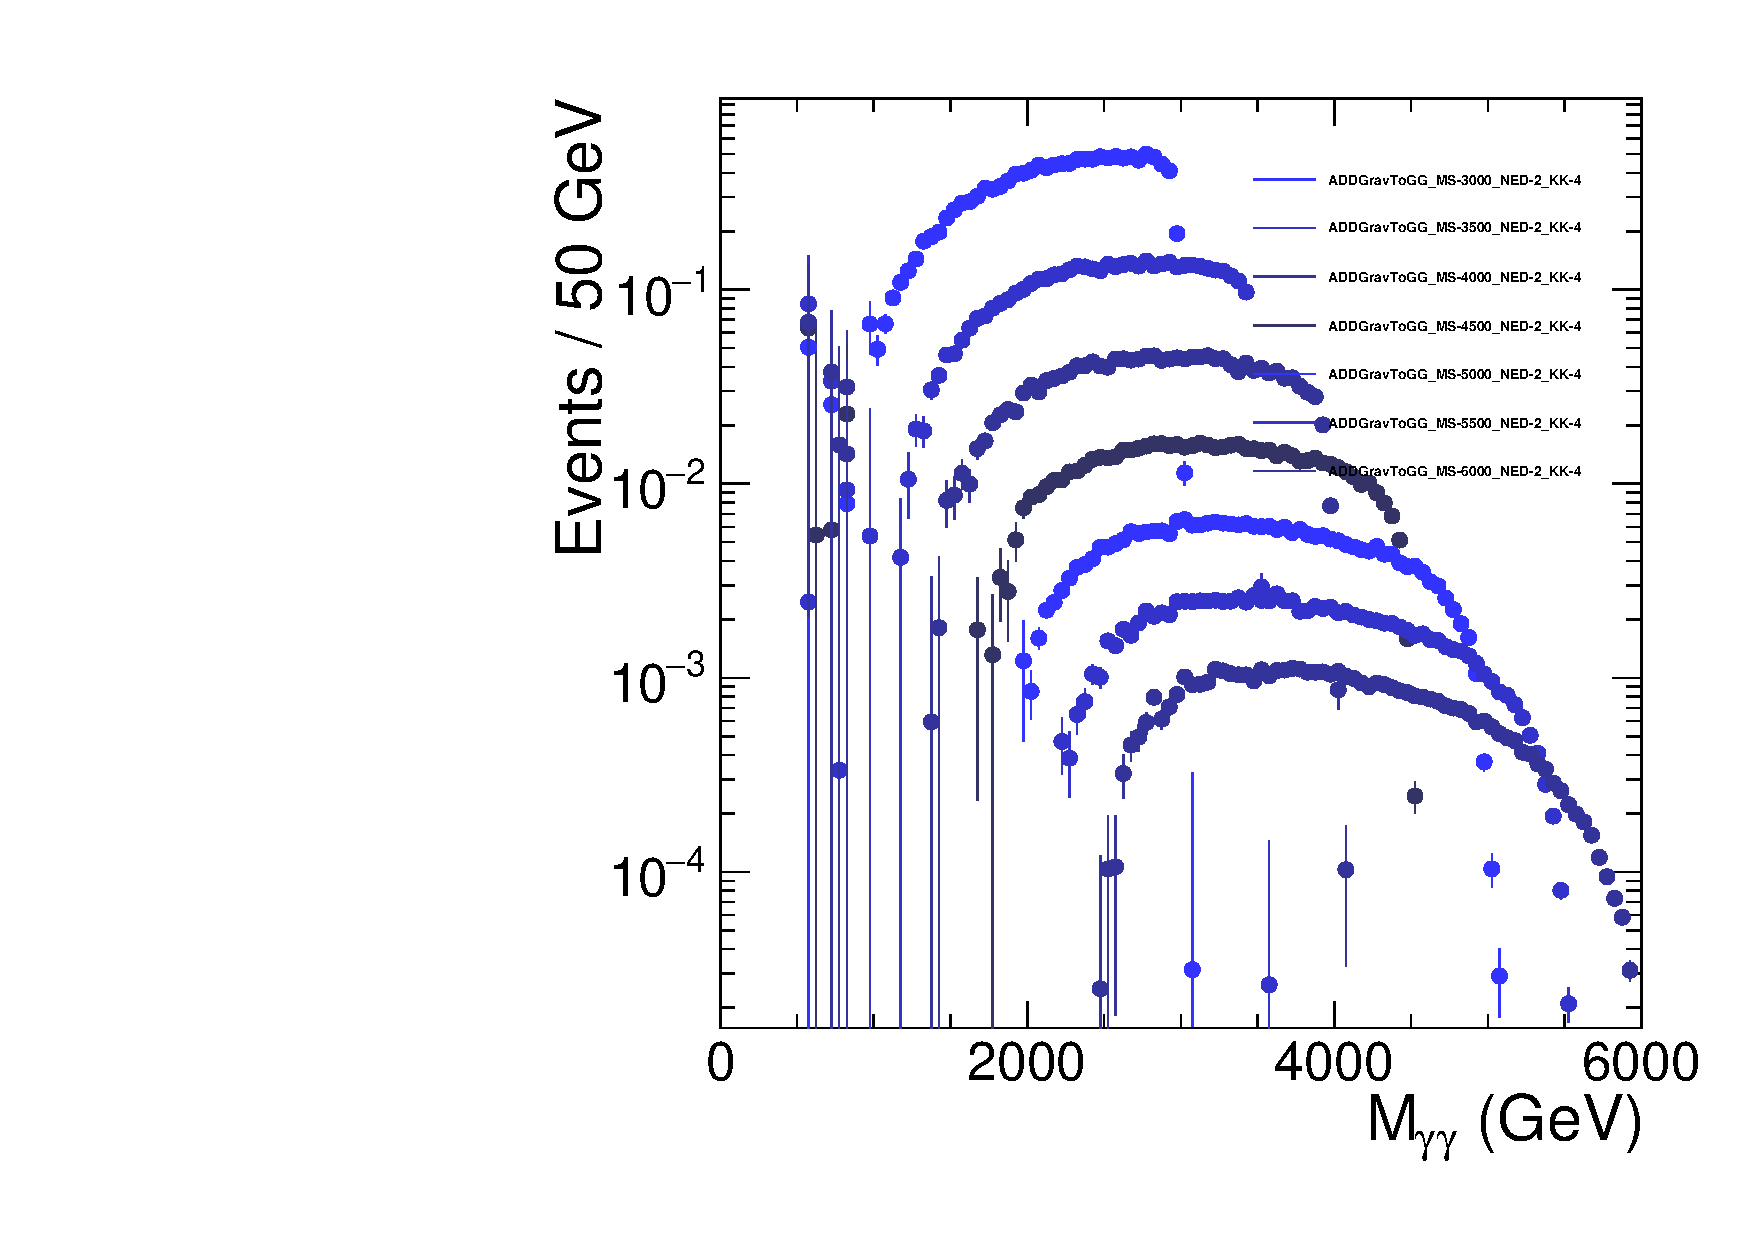
\includegraphics[angle=0,width=0.41\textwidth]{figures/ADDGravToGG_NED-2_KK-4_bkg_sub.pdf}
	\caption{The \Mgg distribution in signal events for the generated values of \Ms before (left) and after (right) subtraction of the SM background. The \KK conventions used in the plots are HLZ with $\nED = 2$ (top), HLZ assuming $\nED = 4$ (middle), and Hewett\texttt{-} (bottom).}
	\label{fig:signal}
\end{figure} 

\begin{figure}[tbp!]
  \centering
  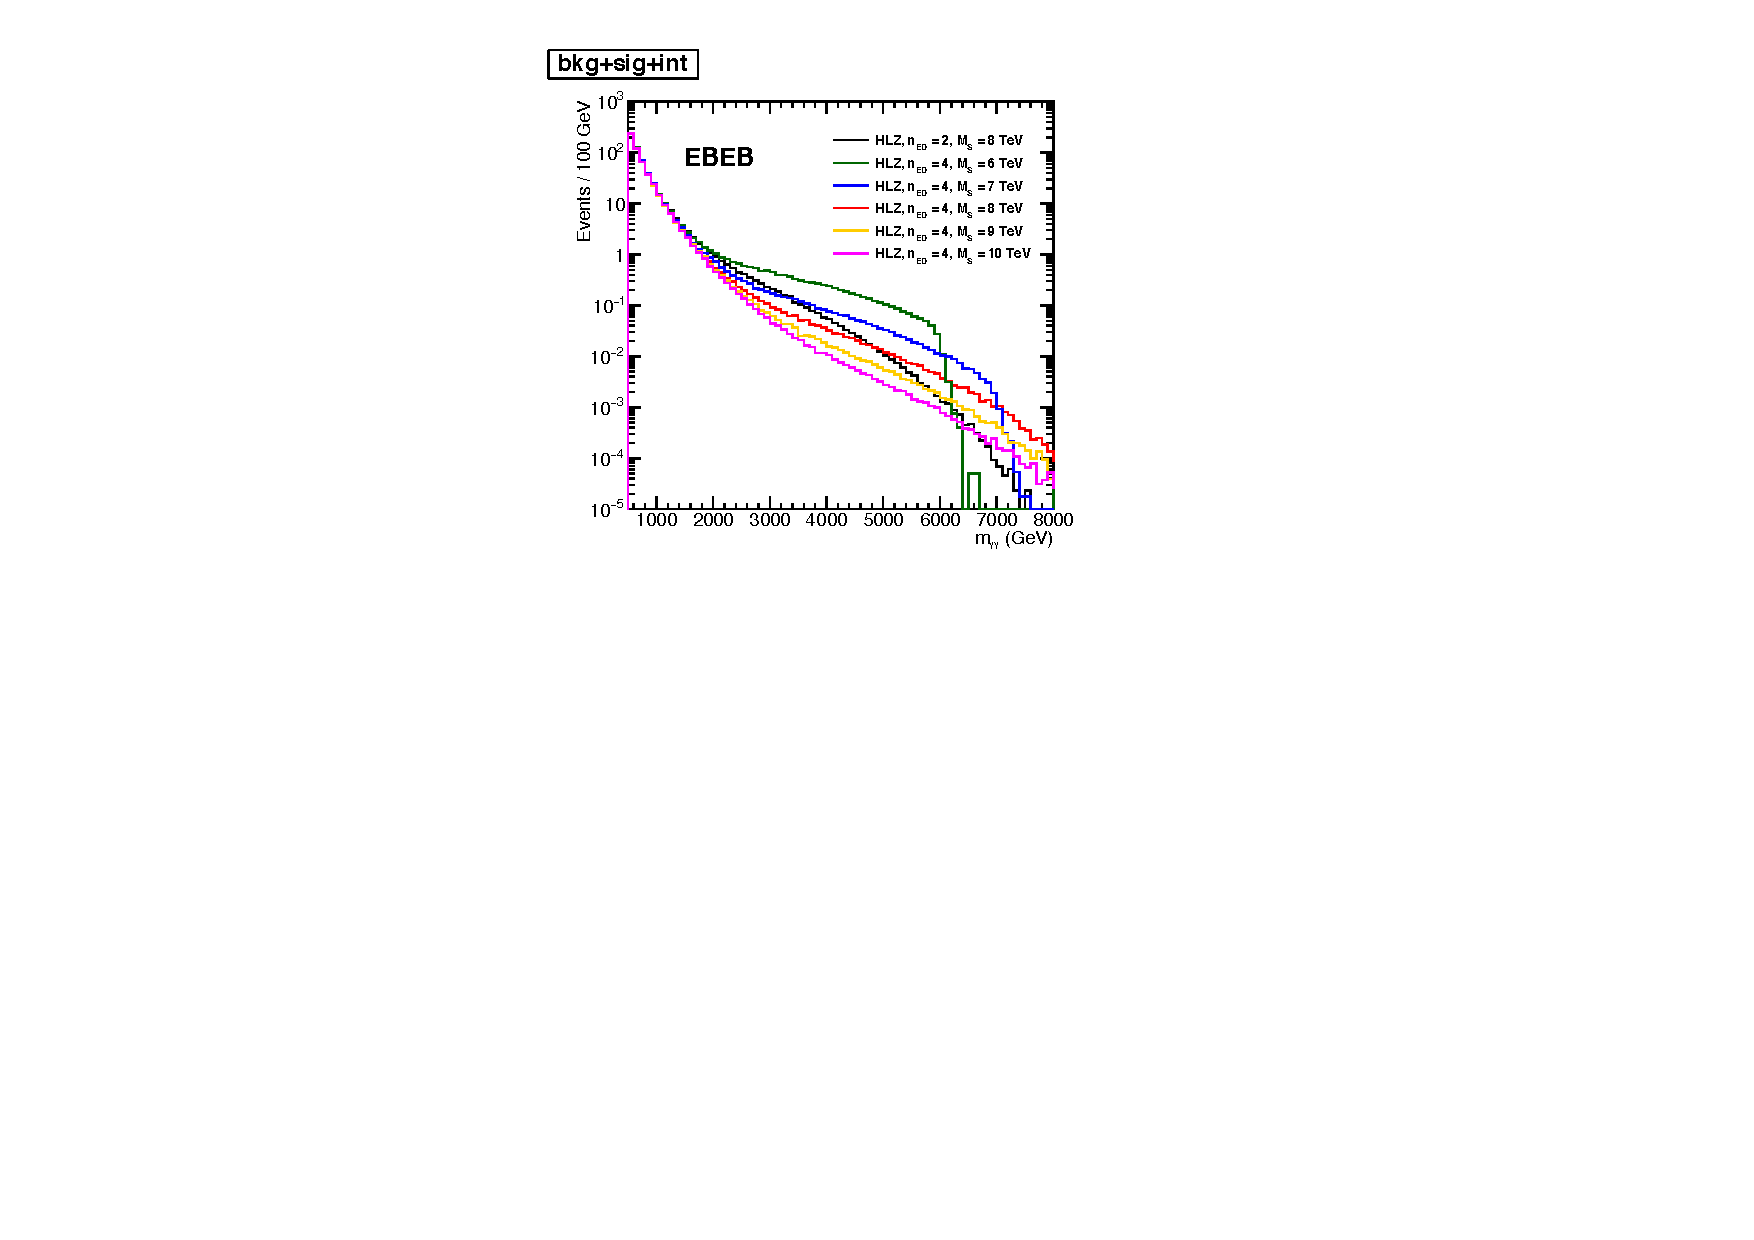
\includegraphics[scale=0.82]{figures/HLZ_sig_int_bkg_left.pdf}
  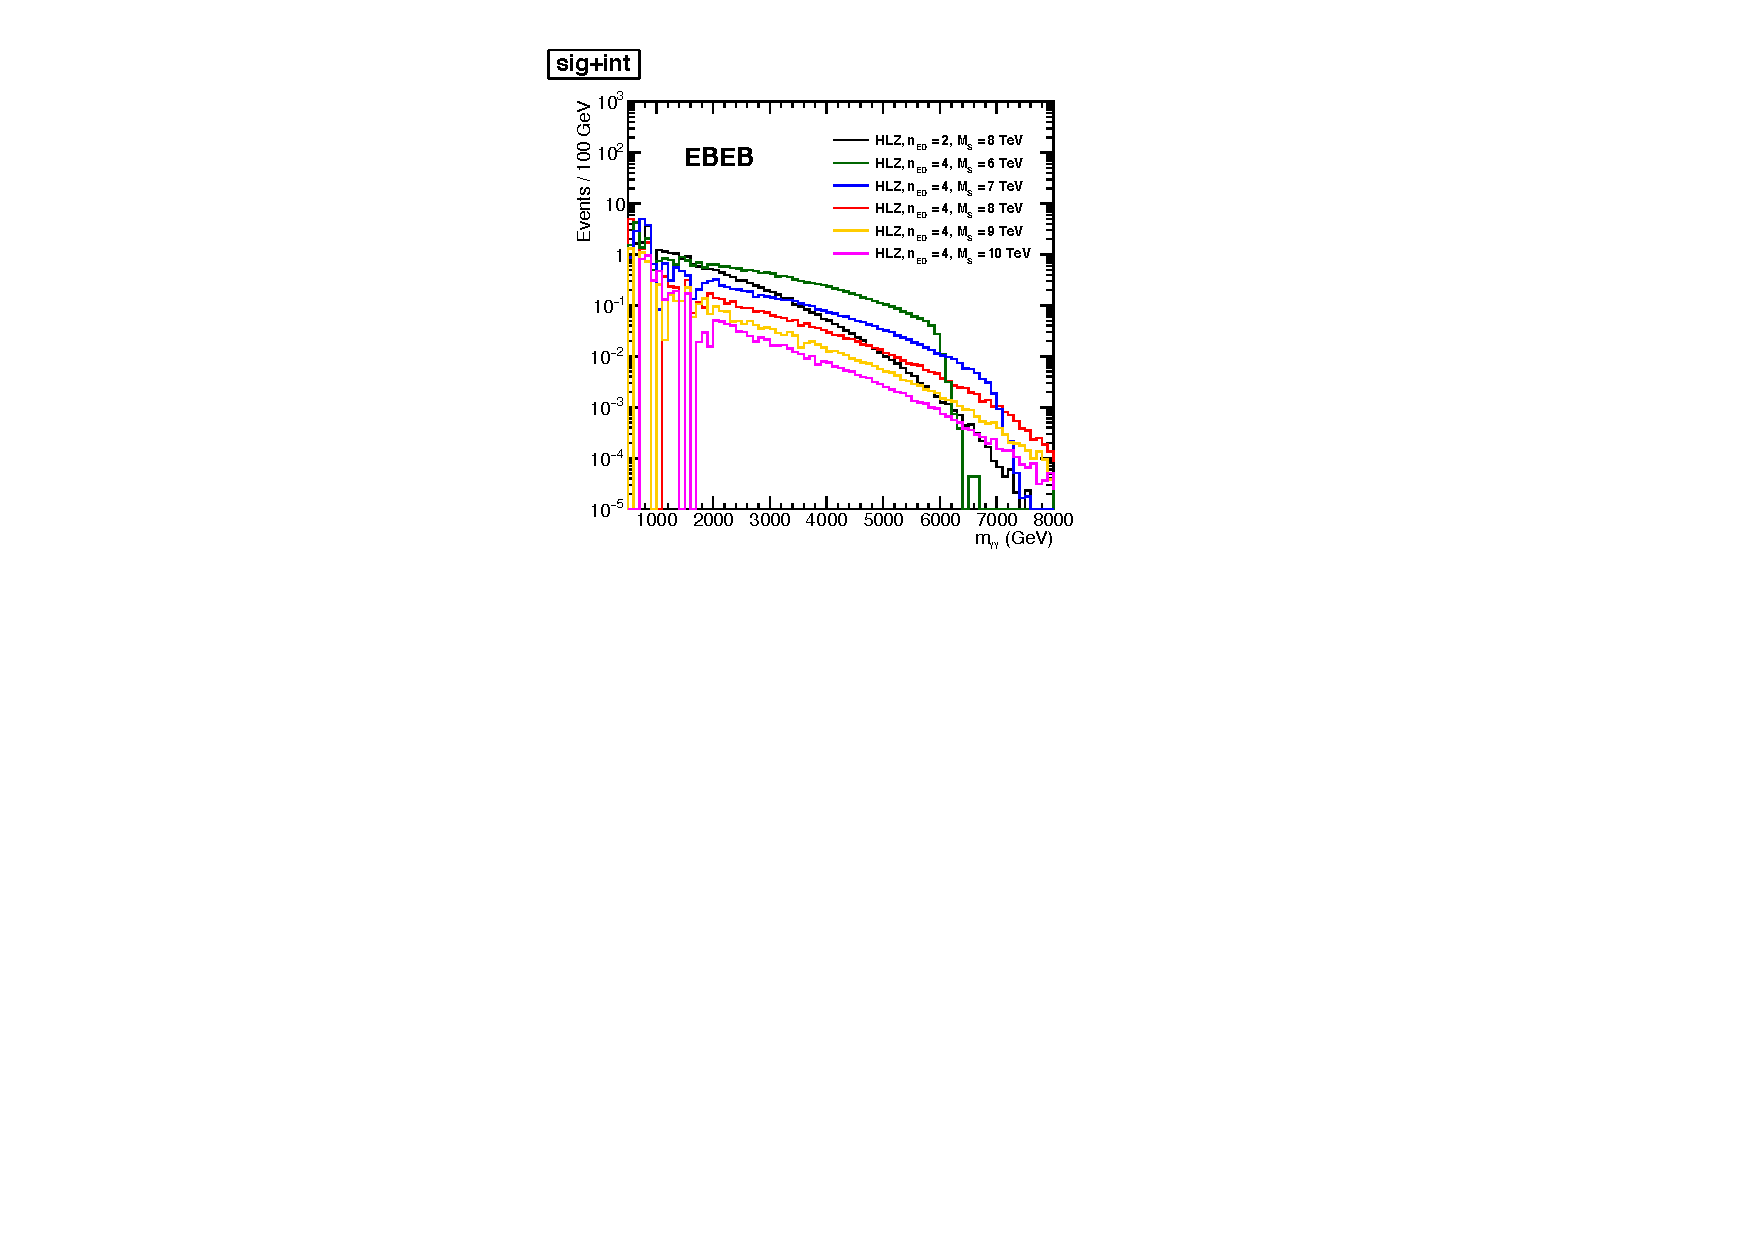
\includegraphics[scale=0.82]{figures/HLZ_sig_int_right.pdf}
  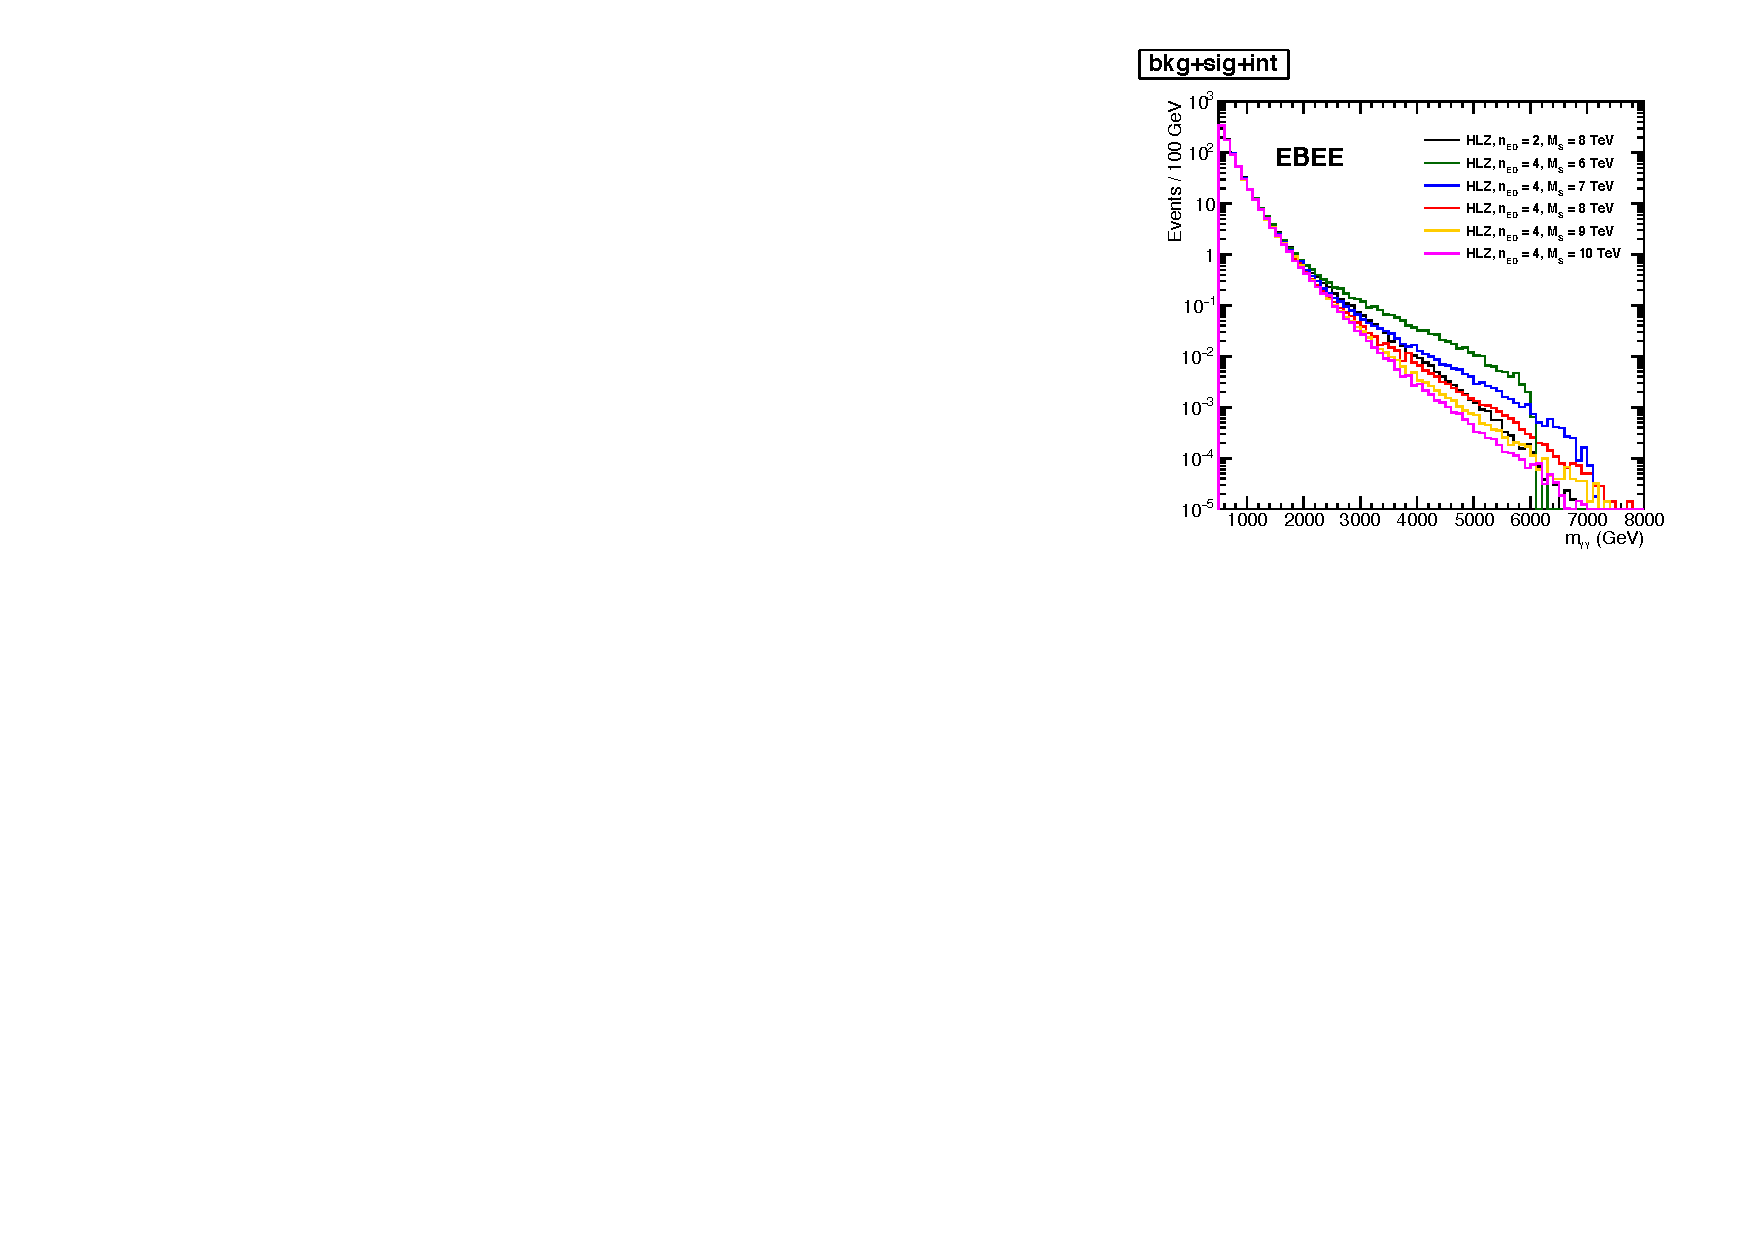
\includegraphics[scale=0.82]{figures/HLZ_sig_int_bkg_right.pdf}
  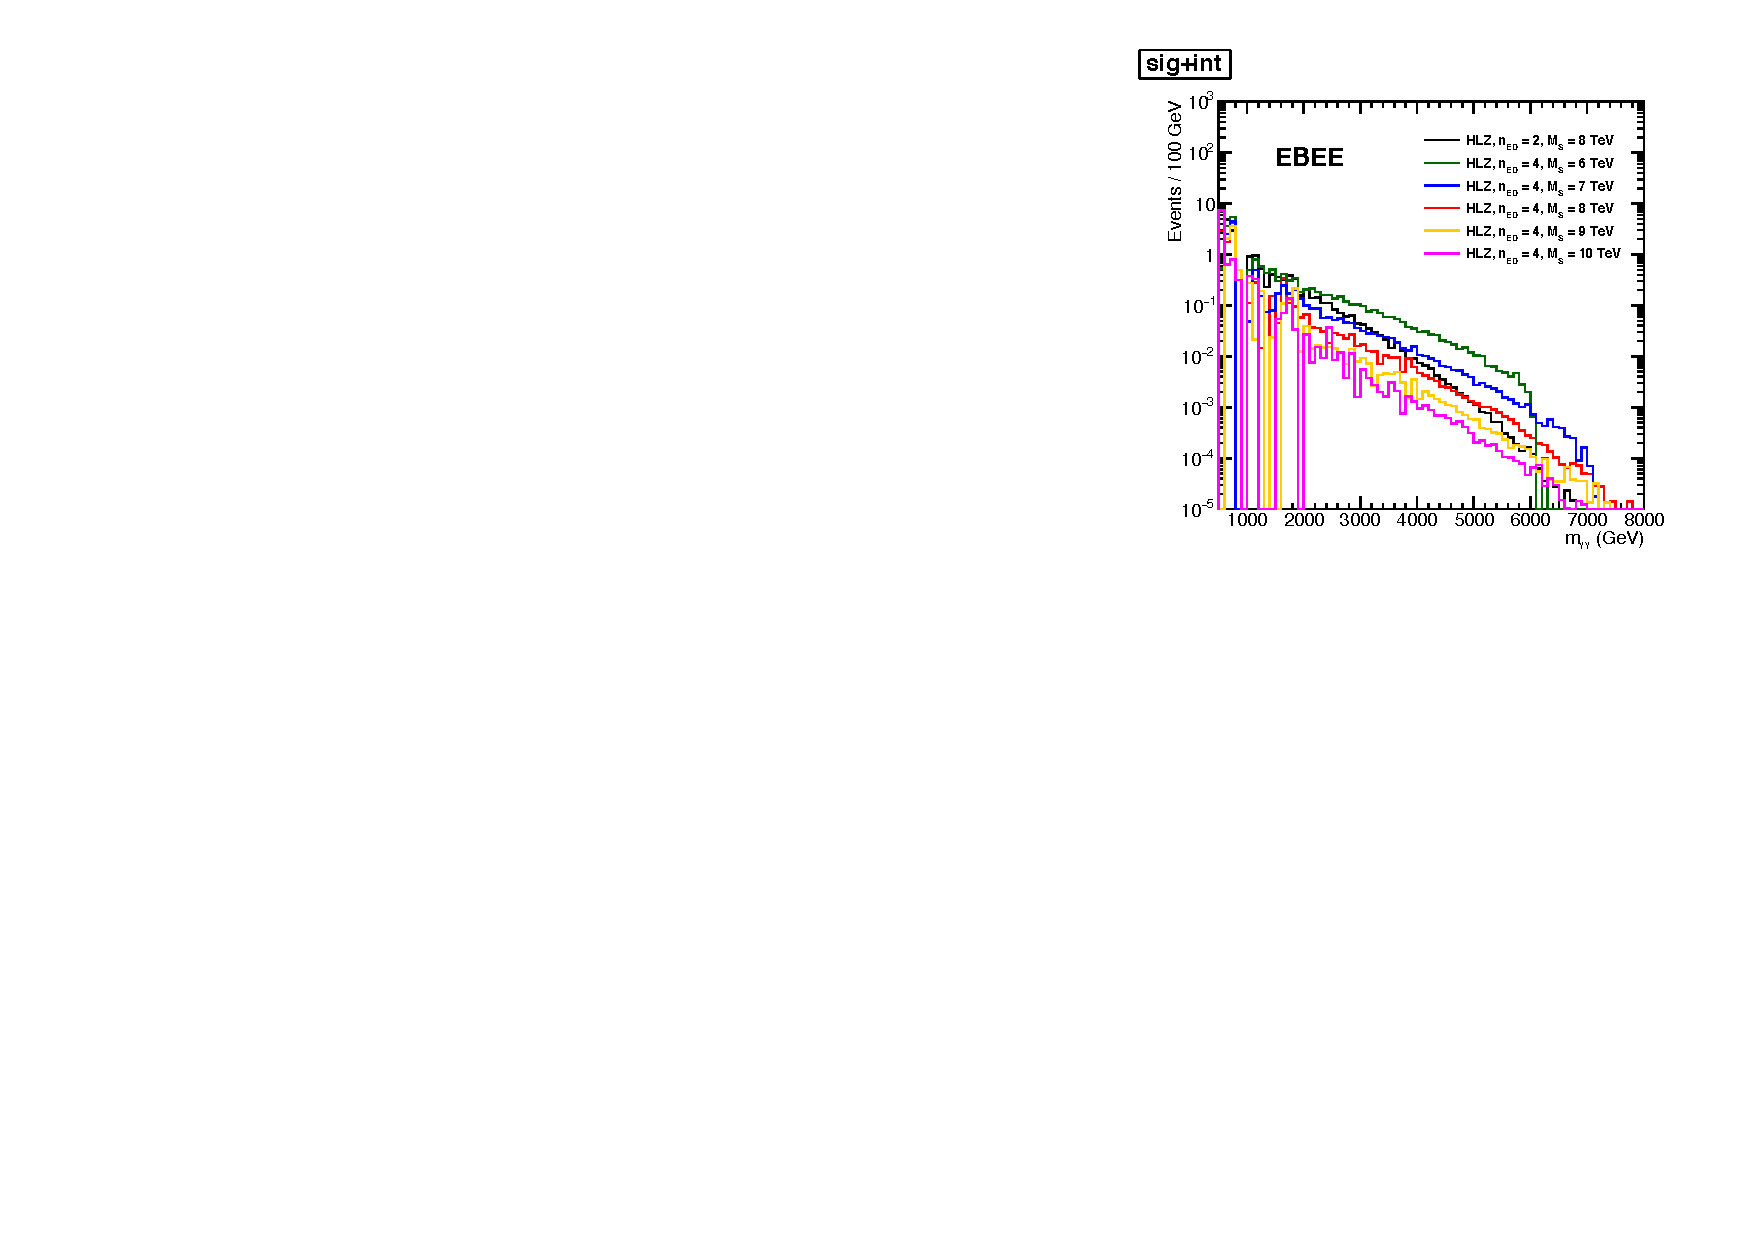
\includegraphics[scale=0.82]{figures/HLZ_sig_int_left.pdf}
  \caption{The \Mgg distributions for the ADD signal and interference before (left) and after (right) subtraction of the SM background in the EBEB (top) and EBEE (bottom) categories. The spectra correspond to the \KK conventions using HLZ with $\nED = 2$ and $\Ms = 8\TeV$ (black) compared against HLZ with $\nED = 4$ using $\Ms = 6$, 7, 8, 9, and 10\TeV.}
  \label{fig:signal_high_Ms}
\end{figure} 

